\documentclass[12pt,a4paper]{article}
\usepackage[utf8]{inputenc}
\usepackage{amsmath,esint}
\usepackage{amsfonts}
\usepackage{amssymb}
\usepackage{geometry}
\usepackage{setspace}
\doublespacing
\usepackage{graphicx}
\usepackage{float}
\usepackage{wrapfig}
\usepackage{caption}
\usepackage{sidecap}
\usepackage{subcaption}
\usepackage{tabulary}
\usepackage{pdflscape}
\usepackage{afterpage}
\usepackage{capt-of}% or use the larger `caption` package
\usepackage[usenames, dvipsnames]{color}
\usepackage{lineno}
\linenumbers*[1]
\usepackage{enumitem}
\newlist{arrowlist}{itemize}{1}
\setlist[arrowlist]{label=$\Rightarrow$}
\usepackage{cite}
%\usepackage{apacite}


\author{Kelian Dascher-Cousineau}
\title{Masters Thesis: The Evolution of Fault Slip Surfaces with Cumulative Displacement}


\begin{document}

\maketitle


\begin{abstract}

Fault slip surface roughness determines fault strength, friction and dynamic fault processes. Wear models and field observations suggest that roughness decreases with cumulative displacement. However, measurements have yet to isolate the effect of displacement from other possible controls, such as lithology or tectonic setting. We present an unprecedentedly large fault surface dataset collected in and around the San-Rafael Desert, S.E. Utah, United States. In the study area, faults accommodated regional extension at shallow 1 to 3 $km$ depth and are hosted in the massive, well sorted, high porosity Navajo and Entrada sandstones. Existing detailed stratigraphic throw profile provide a maximum constraint for displacement. Where cross-sectional exposure is good, we measure exact displacement imparted on slip surfaces using offset in marker horizons. Thereby, we isolate for the effect of displacement during the embryonic stages of faulting (0 to 60 $m$ in displacement). Our field observations indicate a clear compositional and morphological progression from isolated joints or deformation bands towards smooth, continuous and mirror-like fault slip surfaces with increasing displacement. To quantify these observations, slip surfaces were scanned with a white light interferometer, a laser scanner and a ground based Lidar. Together these instruments resolve more than eight decades of spatial bandwidth (from less than $\mu m$'s to $m$'s in scale). In so doing, to the best of our knowledge, we increase the existing data on published fault topographies by XXX fold (available HERE). Results indicate that roughness as defined by the power ($P$) at a given wavelength ($\lambda$) decreases with displacement ($D$) according to a power law, $P(\lambda) \varpropto D^{0.6 \pm 0.1}$. Trends are however subject to significant scatter. Roughness measurement associated with only maximum constraints on displacements corroborate this result—for a given displacement, minimum roughness is bounded by the later smoothing trend. In addition, we find that the maximum roughness is fixed—bounded a by a primordial roughness corresponding to that of joints surfaces and deformation band edges. Building upon our results, we propose a wear model to explain the evolution of faults with displacement. The basis of the model is supported by numerical simulations of crack initiation and growth using boundary element models Fri2D and growth by work-minimization (GROW). Our modelling provides the first insight into fault slip surface process consistent with observational constraints, i.e. fractal geometry and a nearly power-law decay with displacement, by using calling upon scale dependent strength, strength heterogeneity and scale invariant asperity failure by truncation.

\end{abstract}

\section*{Contribution of Authors}

\section{Introduction}
\subsection{Context}
	Faults are a characteristic feature of the Earth’s brittle crust. Crustal permeability, seismicity, and mineralization are just few systems upon which faults act as major controls \cite{sibson1977fault, sibson1994crustal}. In spite of their importance, some aspects of faults and their underlying processes remain poorly understood. What are the frictional properties of faults? How strong is a fault? How do faults mature as they evolve from small to large displacement structures? Key factors such as pore pressure \cite{hubbert1959role, byerlee1990friction}, mineral composition \cite{summers1977note, chester1993internal, holsworth2001structure} and fault architecture \cite{chester1986implications, chester1987composite} have been shown to have important roles in the behavior of faults. However, these factors often fail to explain the highly heterogeneous, chaotic and hierarchical behaviour of faults. Complex fault geometry has long been proposed as a key factor in the faulting process. However, a detailed and robust exploration of the implications thereof has only recently garnered increasing attention. This change of pace maily owes to advances in mathematical theory behind compplex natural systems \cite{mandelbrot1984fractal, mandelbrot1985self}, rapid advances computational abilities enabling more complex source models, thechnological advances in high resolution surveying tools (GPS, photogrametry and Lidar) and detailed field studies of fault architecture  \cite{scholz1986fractal, candela2012roughness}. Fault geometry has since been included as a key component of wholistic explanations for the  mechanical behavior and evolution of faults (e.g. \cite{lay1982asperity, aki1984asperities, scholz1986fractal}). 


	Fault zones generally comprise of a damage zone and fault core. The damage zone represents the haloe of subsiduary fault features including smaller fault, fractures, cleavage and veins. The fault core generally represents the zone in which most of the dispalcement has taken place and is associated with intense comminutions of the protoloth  \cite{sibson1977fault, chester1986implications, caine1996fault}. Actual Slip on a fault occurs on discrete slip surfaces within the fault core \cite{palmer1973growth, engelder1974cataclasis, aydin1978development, sibson2003thick}. These surfaces are not planar; they are rough \cite{scholz1986fractal}. Slickenlines, corrugations, mullions and jogs are all fault slip surface features which reflect the multiscale nature of fault roughness \cite{scholz1986fractal,sagy2009geometric}. Field studies have found common characteristics in the statistical properties which describe the topography of fault surfaces. These can be summarized as follows: 1) Fault surfaces topographies appear to be well defined by large fractal domains \cite{scholz1986fractal} , wherein 2) faults are smoother at larger length scales  \cite{schmittbuhl1993field, andela2012roughness} and 3) are rougher in the slip-perpendicular direction than in the slip-parallel direction \cite{schmittbuhl1993field, lee1996structural}.
	
	Fault roughness has been demonstrated to be critical in determining fault properties and corresponding scaling relationships. A series of field investigations, laboratory experiments, analitycal predictions and numerical simulation have explored the heterogeneous stresses and deformation patterns around complex fault geometries around single fault steps, ramps and jogs (e.g. \cite{berger1980first, segall1980mechanics, mcclay1987analogue, kilsdonk1989analytical, burgmann1994slip}), on simple theoretical fault geometies (e.g. \cite{chester1997stress, chester2000stress}), and real or sythetic faults with geometrically fractal bandwitdths in two dimensions (e.g. \cite{saucier1992stress, griffith2010rough, dunham2011earthquake, ritz2015influence} and three dimensions (e.g. \cite{okada1992internal, meade2007algorithms, shi2013rupture, zielke2016sub, zielke2017fault}). Direct repercussion of complex stress patterns include the following: increased geometrical shear resistance \cite{fang2013additional}; increased and spatially variable off-fault damage and fracture energy \cite{okubo1984effects, chester2000stress, griffith2010rough}; reduced stress drop \cite{zielke2016sub} and impeded slip budjet \cite{dieterich2009nonplanar}. In numerical simulations, \citet{zielke2017fault} reports a nearly two-fold decrease in earthquake moment release for a fault with realistic roughness compared to its planar counterpart. Laboratory experiments comparing smooth and rough surfaces show that with increasing roughness, friction increases \cite{biegel19921}, rate and state $a-b$ slip stability increases \cite{marone1994scaling}, critical slip distance increases and rupture nucleation dimension increases with surface roughness \cite{okubo1984nonplanar}. These features do appear in earthquake statistics. For example, bolstered by numerical simulations of complex stress fields, Parsons, 2008, found that persistent clusters and gaps in seismicity can be attributed to geometrical complexities on faults.
 
It is therefore increasingly evident that roughness is both a fingerprint of the fundamental features of- and an active agent in the faulting process \cite{scholz1986fractal, brodsky2016constraints, candela2011stress}. In accordance, incorporating more complex sources geometries has become a more frequent practice in forward and inverse dynamic earthquake rupture modelling (e.g. \cite{shi2013rupture, moreno2009impact, zielke2016sub}.

The measured magnitude of roughness is highly variable from one fault to the other. While there has been significant progress in understanding the active role of roughness in the faulting process, it remains unclear what determines the complexity of fault geometry (e.g. \cite{candela2012roughness, brodsky2016constraints}). Sagy et al. (2007) noted a systematic decrease in roughness of ‘mature’, large displacement faults compared to ‘immature’ faults with low displacements. Similar results have been observed along reactivated joints, in laboratory experiments \cite{davidesko2014evolution}, and in compilations of fault roughness analysis \cite{brodsky2011faults, candela2009characterization}. However, these data show only weak correlations between fault roughness and cumulative displacement \cite{brodsky2011faults, candela2012roughness}. These results are also put in question by later experiments showing roughening with shear with normal loads higher that 7.5 MPa \cite{badt2016geometrical}. Detailed qualitative field investigation have further shown that slip geometry arises from net process between smoothing (i.e. asperity failure and wear) and re-roughening (e.g. off-fault damage) \cite{shervais2016smoothing}.

If fault geometry changes as a fault accumulates displacement, it would have a profound effect on fault mechanics and, correspondingly, seismology. However, relating fault roughness to cumulative displacement is not trivial. Experiments cannot perform tests with realistic roughness over large enough displacement. It is also unclear how laboratory experiments scale up to natural faults because of the fractal scaling exhibited by natural fault systems. Exhumed fault slip surfaces are rarely well preserved. In the field, obtaining well-constrained displacement estimates is contingent on the presence of precise and accurate kinematic indicators (e.g. piercing points). Additionally, combining observations over a broad range of displacements is challenging. Consequently, it is unclear whether trends observed in compilations of roughness measurements from multiple faults are directly attributable to displacement or a combination other geological factors \cite{brodsky2011faults}. For instance, while comparing fault surfaces from geologically diverse datasets, variations in lithology, faulting regimes, temperature and depth may all be introducing further systematic variations. 

The existence of a distinction between mature and immature faults and the precise characterization of this transition has far-reaching implications. As discussed above, earthquake sources parameters are sensitive to fault roughness. Correspondignly, an evolution of roughness with displacement implies that "not all fault should be treated equally". This prediction is consistent with more efficient energy radiation measured on mature faults compared to immature faults \cite{harrington2009smooth}; and changes in b-values associated with fault off-set \cite{stirling1996fault}. Additionally, the evolution of roughness would have a corresponding effect on the architecture of a fault zone.  The geometry of the fault surface modulates the architecture of the whole fault zone \cite{chester2000stress, griffith2010rough, ritz2015influence}. Changes in roughness require interaction between the slip surfaces and its direct surrounding (fault core), resulting in the formation of fault rock \cite{power1988roughness} and off-fault damage \cite{griffith2010rough, ritz2015influence}. The co-evolution evolution of the fault slip surface and the fault zone as a whole is a novel insight the maturity of fault from a structural point of view.
	
\subsection{Fault Roughness}

The deviation of fault surfaces from planarity formally defines roughness \cite{brown1985broad}. Pioneering studies used contact profilometers to measure the roughness of fracture and fault surfaces along  dirscete profiles \cite{mandelbrot1984fractal, brown1985broad, scholz1986fractal, power1987roughness, power1991euclidean}. Combined with the surface profile of the San Andreas fault, faults were found to exhibit fractal scaling over a remarkably broad range of length scales ranging over 10 orders of magnitude—from $10^{-5}$ to $10^5 m$ \cite{scholz1986fractal, power1987roughness, aviles1987fractal}. Over these length scales, fractal scaling is said to be statistically self-affine \cite{mandelbrot1984fractal, mandelbrot1985self}. 
	
A statistically self-affine profile along $x$ with heights $h(x)$, is invariant under the affine transformation:

\begin{equation}
\left\lbrace
  \begin{matrix}
   	x \rightarrow \lambda x \\
    h \rightarrow \mu h
  \end{matrix}
\right\rbrace
\end{equation}


This relation therefore implies an exponential relation between the scaling, $\lambda$ (along $x$), and $\mu$ (along $h$) such that:

\begin{equation}
\mu = \lambda^\varsigma
\end{equation}
%
Where $\varsigma$ is a constant named the Hurst exponent \cite{schmittbuhl1993field}.

Many analytical methods exist to quantify the fractal roughness of faults \cite{mandelbrot1985self, schmittbuhl1995reliability, candela2009characterization}. Possibly most intuitive of these methods is the Root Mean Squared ($RMS$) as a function of scale. It is effectively a measure of topographic variance. For a given profile of length $L$ with a point spacing of $\Delta x$ with deviation $h$ from the best fit line, the $RMS$ is defined as follows:

\begin{equation}
RMS(L)=\sqrt{\dfrac{\Delta x}{L}\sum^{L/{\Delta x}}_{i=1} h^2_i}
\end{equation}

	The $RMS$ roughness of a fault or fracture exhibits a positive power-law scaling with segment length. A self-affine profile should therefore plot as a straight line on a log-log plot of the $RMS$ as a function of the segment length with a slope equivalent to the Hurst exponent \cite{schmittbuhl1995reliability}.
	An alternative approach to describe the fractal roughness of faults has instead been the power spectrum and variations thereof (i.e. amplitude spectrum and power spectral density). By testing various fractal analitical tools on synthetic profiles \cite{schmittbuhl1995reliability} and surfaces \cite{candela2009characterization}, the power spectral analysis was shown to yield estimated of scaling exponent most robust to system size and Hurst exponent values.
	 For a set of discretely sampled points, the power spectrum of a profile is the result of a Fourier transform. In practice it is obtained using a Fast Fourier Transform algorithm (FFT). The power spectrum describes a two dimensional surface profile as linear superposition of sinusoidal profiles discretized over a fixed frequency domain. In the frequency domain, rougher profiles will have correspondingly higher amplitudes, or power. The power spectrum of a self-affine profile defines a power-law:

\begin{equation}
P(k) = Ck^{(-1-2\varsigma)}
\end{equation}

Where $P(k)$ is the power at a given spatial frquency, $k$, $C$ is the pre-factor and $\varsigma$ is the Hurst exponenet \cite{mandelbrot1985self, power1991euclidean, schmittbuhl1993field, candela2012roughness}. 

Early studies suggested that fault surfaces were approximately self-similar. Self-similarity represents a self-affinity with a Hurst exponent is 1 \cite{mandelbrot1985self}. The developments in laser scanner technology over the past decade, particularly terrestrial laser scanners, enabled the detailed charachterization of slip surfaces in three dimension \cite{lee1996structural, kokkalas2007quantitative, renard2006high, sagy2007evolution, sagy2009geometric, jones2009quantitative, bistacchi2011fault, brodsky2011faults, candela2012roughness}. Later studies averaging cross-sectional profiles through a fault surface suggested that smaller Hurst exponen less than 1 may better characterize fracture surfaces and faults (e.g. \cite{schmittbuhl1993field, lee1996structural, sagy2009geometric, candela2012roughness}). Studies of natural mode I crack surfaces have observed radially sym self-affinity with a Hurst exponent of $\sim$0.8 at all scales of observation (\cite{schmittbuhl1995scaling, bouchaud1997scaling}-and references therein). Shear, or mode II cracks (i.e. faults) were found to differ in that they are anisotropic. The Hurst exponent parallel to shear ($\sim$0.6) is smaller than that in the shear-perpendicular direction ($\sim$0.8) \cite{lee1996structural, sagy2007evolution, bistacchi2011fault, candela2012roughness}. Overall, observations also show that fault surfaces have distinctly smoother profiles along slip direction than perpendicular to slip \cite{lee1996structural, sagy2007geometric, candela2012roughness}. The magnitude of the roughness in both directions is, however, subject to a substantial spread in values over many orders of magnitude \cite{candela2012roughness, brodsky2011faults}. This variability is most strongly reflected in the pre-factor. Recent studies also report a minimum length scale of grooving, a length scale at which slip surface is no longer anisotropic \cite{candela2016minimum, brodsky2016constraints}. This transitions typically occurs around 4 to 500 $\mu m$ and roughly corresponds to where the fractal scaling in the slip parallel and slip perpendicular direction meet.

Why are slip surfaces fractal? The fractal character of slip surfaces can be explained by a range of processes. There is, however, no clear consensus in the existing literature. Candidate explanations include the superposition of random wear processes processes, random fracture tip growth, and more ... Perhaps most topical is the proposition of scale dependent strength as proposed by Brodsky et al., 2016. Using the aspect ratios of geometrical asperities as a measure of rock strength at a given scale, it is argued that fractal character of fault surfaces directly reflects a scale dependence in rock strength. Moreover, a break in fractal scaling at the $\approx XXX \mu m$ length scale is interpreted as a transitions from inelastic or brittle processes (large scales) to plastic processes. This explanations is in agreement with laboratory experiments that report that larger volumes of rock are, on average, weaker ...

Fractal characterizations of surfaces do not uniquely define a profile or surface. Other statistical metrics exist and are common place in many engineering practices. Specifically, examining the statistical distribution of the height measurements of a surface provides insight into the contact \cite{greenwood1966}, frictional behavior \cite{XXX} and wear processes \cite{archard1953contact}.

define skewness, kutosis, etc.

The the statistical moment is defined as follows:

First ($m=1$) and second ($m=2$) order  



\subsection{The evolution of slip surfaces with displacement}

*this could be in an interpretation section

Previous work has mainly assotiated fault surface deformation to mechanical wear processes as the dominant mechanism of surface evolution \cite{power1988roughness, sagy2007evolution, brodsky2011faults}. Mechanical wear processes include any erosive process in which volume removal is frictionally induced from surfaces in sliding contact. Before further exploring the effects of wear in fault slip surfaces, it is worth recognizing that many other processes could--and likely do--cause the slip surface to evolve with displacement.

A surface can change according to the following:

\begin{itemize}
	\item[] \textit{surface deformation}
	\item[] \textit{Addition of material}
	\item[] \textit{Removal of material}
\end{itemize}

Fault slip surfaces have evidence pointing to each of these processes preserved in the rock record.

\textit{Surface deformation} encompasses any process by which a surface changes shape by the rearrangement of material (no removal or addition). Both elastic and inelastic processes allow fault blocks to deform. At the seismic time-scales, only elastic and brittle deformation can occur--whereby macroscopic fault damage and micro-fractures in grains and crystals away from the fault can enable stain and dissipate stress on the fault. At longer time-scales, calcite twinning, pressure solution, and clay alteration can also occur yield similar effects. These short and long-time scale mechanisms define the visco-elastic rheology of fault blocks.

It is unlikely that the rheology of the fault block and its effect on the slip surface topography are significant in the evolution of the slip surface. Using slickenline orientations and fault core thickness as a proxy to the fault block rheology Kirkpatrick et al. 2014, find that 1) deformation does occurs in fault block and 2) there is a scale dependence to this deformation whereby. However, this scaling is not well represented in fault geometric scaling. It would rather predict a change in scaling at the outcrop scale. The absence of any such signal in the topography of fault slip surfaces implies that deformational processes cannot directly determine how slip surfaces evolve with displacement.

For its part, an \textit{addition of material} occurs as fault rock is cemented onto slip surfaces--filling in geometrical concavities and effectively reducing the amplitude of surface irregularities. Its effect is preserved in the rock record with mobile, or \textit{fluidized}, gouge cemented and re-fractured in subsequent faulting \cite{sagy2009geometric, shervais2016smoothing}. Moreover, it has been shown that discrete slip surface can arise from the localization of shear strain within unconsolidated granular material (e.g. \cite{chambon2006thickness}). It is key to note that this, and similar, mechanisms are then metered by the healing-rate and the wear-rate.

\textit{removal of material} is caused by mechanical wear. As fault blocks slide past each other, frictional wear is an inevitable process. Layers of comminuted fault rock, cemented or not, are direct evidence of this process \cite{power1988roughness, scholz1987wear}. Wear is known to be multiscale. At small scales, grains can be plucked or broken \cite{shervais2016smoothing}; at larger scales grains plough slip surfaces to crear corrugations \cite{scholz1976role} and sidewall ripouts form \cite{swanson1989sidewall}. It is key to note that 1) all these processes fall under the definition of wear in that the involve the failure of geometrical protrusions, only these are expressed at various scales and 2) these have substantive impact on the surface geometry.

MAKE FIGURE HERE FOR REFERENCE SIMILAR TO THE ONE IN YOUR EPSL SLICKENLINE/RHEOLOGY PAPER - but focus on the fact that there is an asperity failing. 

While wear processes are subject of a vast field of research, particularly in engineering and tribology due to interest in manufacturing machine parts for longevity \cite{meng1995wear}, its  applications in the earth sciences is emergent with tests mainly conducted at laboratory scales \cite{power1988roughness, scholz1987wear, wang1994wear, rathburn2013Numerical}. The only applications to natural fault surfaces is a prediction of wear volume presented in Brodsky et al., 2011. 

The wear rate, the volume of wear-product produced per unit offset is broadly related to the real area of contact and loading. When two surfaces are put in direct contact, the real area of contact is much smaller than the nominal surface areas because the load is supported at microscopic protrusions from a surface, or \textit{asperities} (\cite{archard1953contact, greenwood1966contact, bowden2001friction, dieterich1996imaging}). Remote loading normal to the surface causes local stresses and associated deformation at contact points. Note that as the load is increased, deformation of large asperities causes new asperities to come in contact. In its simplest form, wear rate ($\dfrac{\partial V}{\partial x}$) is defined according to defined to be proportional to the remote load ($P$):

\begin{equation}
\dfrac{\partial V}{\partial x}\varpropto P
\end{equation}

The relation has been shown to be reasonably robust in experimentation for most materials. In further detail, the size, distribution and duration of contact areas, as well as the shape of the worn particles, control the general behaviour of wear. Note that material properties are contained in a constant of proportionality referred to as the probability factor—the probability of a collision of asperities to lead to removal of material \cite{archard1953contact}.

	Following this formulations, Scholz, 1987, proposed that wear rate for faults could be determined as a linear relationship with displacement and an inverse relationship with hardness. The displacement relationship is in reasonable agreement with laboratory experiments \cite{yoshioka1986fracture} and measurements of natural fault rock thickness \cite{robertson1982continuous, shipton2006thick}. The hardness dependence is difficult to test given uncertainties in both fault rock thickness and hardness \cite{scholz1987wear}. The simple formulations forwarded by Archard, 1953, and its application to faults by Scholz, 1987, was aknowledged to have serious limitations in their applications to natural faults. Specifically, the author raises concerns about the surface geometry of real fault, and about the scaling and effectiveness of wear processes such as grains plucking and fault rock abrasion.

   Building off of experiments on engineering metals \cite{queener1965transient} and ceramics \cite{levy1988unlubricated}, new fault wear model integrated a 'running-in' component which exponentially decays towards steady-state \cite{power1988roughness, wang1994wear}. This behavior intruced a discrete such that the volume of fault rock produced ($V$) can be expressed as a function of displacement ($x$) according to:
   
\begin{equation}
   V = \beta \left[ 1-\exp(-nx)\right] +Kx
\end{equation}
%
Where $\beta$, $n$, and $K$ are constants. 

	A running-in stage is though to reflect effect of surface roughness. This later formulations was supported by a semi-analytical formulations of asperity failure and rotary shear experiments. However, in line with comments in Power et al., 1988, we propose that this running-in stage on real faults is likely to be substantially different for faults where fractal topography implies that new larger asperities will come into contact with increasing displacement. Laboratory experiments have limited fractal bandwidth. Shear boxes are limited to sample length; rotary shear apparatus are limited to their circumference length. We highlight that wear processes controlling the behaviour laboratory scale experiments are likely inadequate for natural faults. These may instead reflect relict behaviour issuing from limited fractal bandwidth and emplacement of mobile gouge layers buffering the surfaces.
   
%	If and how wear affect the geometry of a fault slip surface remains unclear. Both field and laboratory experiment show that wear is scale dependent, such that asperities are worn down at different rates according to their typical dimensions. Asperities at longer characteristic wavelengths and larger amplitudes wear down faster, on average, than those with small wave lengths and small amplitudes. The exact mechanism causing this behavior is unclear. Davidesko et al., 2014 suggest that dilation during displacement on a fault ‘shelters’ smaller, shorter wavelength, asperities and therefore wears down large, long wavelength asperities.

It is clear that the fractal nature of fault surfaces is important to reconcile with a model of wear. Concepts of fractal scaling, strength heterogeneity and scale dependent strength are poorly captured by the current literature. Additional insight from field observations are needed to better understand fault slip surface processes. To date, notwithstanding preliminary efforts by Brodsky et al., 2011, linear scaling between fault rock thickness and displacement is nearly the only grouding field evidence for existing wear models (i.e. \cite{scholz1987wear, wang1994wear, power1988roughness}). As pointed out by many authors \cite{blenkinsop1989thickness, evans1990thickness, shipton2006thick} the scaling is contingent on highly uncertain and ambiguous measurements. Overlooking difficulties and/or inconsistencies in determining displacement, the representative fault rock thickness is difficult to measure given variations of in thickness (often many orders of magnitude, even for a single outcrop), inconsistent definitions of the measurements across the literature, and potential breaks in scaling for certain faults. 

The lack of a model grounded in more field observations, quantitative data and theoretically consistent with our current understanding of fault slip surfaces is a blaring knowledge gap that we seek to fill in this study. 

%These include sensitivity to fault rock, sliding velocity and the presence of lubricant (e.g. pseudotachylyte, amorphous silica gel and gouge). Moreover, the stresses imparted by a propagating fault rupture front are mechanically distinct from those related to rubbing surfaces. Such a distinction may also drastically alter the relation between wear material and the slip surface \cite{sibson1977fault}. Since Archard (1953), models of wear tend to diverge in their results, assumptions and by association, their applicability \cite{meng1995wear}.



\subsection{Faulting in Sandstone}

Faults in the well sorted Navajo and Entrada Sandstones in the San Rafael desert provide an ideal natural laboratory for the study of fault maturation. These have correspondingly been subject of extensive study of fault mechanics (e.g. \cite{aydin1977faulting, aydin1978development, krantz1986orthorhombic, shipton2001damage, shipton2002structural, shipton2003conceptual, fossen1998deformation, fossen2005fault}  \cite{fossen2007deformation}). Its is however important to recognize faulting in sandstones such as the Navajo and Entrada units do have some peculuaritie that are worth outlining. Before presenting the tectonic and geological context of the the San Rafael desert, we first provide a brief overview of the existing litterature covering the nucleation, growth and coalescance of faults in sandstones with a specific focus on the areas presented in this study.

Two fault nucleation models exist faults in sandstone \cite{aydin1977faulting, davatzes2003overprinting}, the first model is based on the localization of strain along deformation bands and deformation band clusters. Deformation bands are a characteristic feature of high porosity sediment \cite{aydin1977faulting, aydin1978development, fossen2007deformation}. Deformation bands define sinuous sheets which localise strain in zones typically less that a few millimetres in thickness \cite{fossen2007deformation}. Strain is accommodated by the run-away crushing of sedimentary grains and the concomitant collapse of pore space. Strain across deformation bands is typically in shear \cite{fossen2007deformation}. Shear strain accommodated across a single deformation band is typically on the order of millimetres. With increasing shear strain, deformation bands coalesce in localized zones called  deformation band clusters. It is characteristic for deformation bands, and deformation band clusters to protrude out of outcrop because of differential weathering. Field studies show that faults form in or along these deformation band clusters \cite{aydin1977faulting}. 

The second nucleation mechanism relies on the reactivation and coalescence of regional mesoscopic joint sets \cite{myers1999structure, davatzes2003overprinting}. Subsequent deformation leads to the formation of additional joints, sheared joints, zones of fragmentation, and, finally, through going slip surfaces enableb be the likage of splay fractures and joints (see figure \cite{fault_nucleation_b}. This faulting mechanism is typically associated with more intense becciation and 

The models have since been shown to be endmembers for the formation of faults in the High porosity sandstone such as that of the Navajo Desert presented in this study . Moreover, these mechanisms can act in unison and result in relatively complex overprinted architectures \cite{davatzes2003overprinting}.

The maturation of faults in the Navajo and Entrada sandstones, and similar units in the region is particularly well recorded. In these units, the formation of pristine, slickensided slip surfaces is common and seemingly does not require large displacement form \cite{aydin1977faulting, aydin1978development}. While the evolution of slip surface with siplacement is not  described in these field area (as will be done in this study), there has been substantial work describing the evolution and growth of damage zones with displacement which report roughly linear scaling laws over 0 to 50 meters of displacement \cite{shipton2001damage, shipton2003conceptual, davatzes2005distribution}. Also, while it was typically though that defomation bands pre-date the formation of faults \cite{aydin1977faulting, aydin1978development}, it was shown that later generations of deformation bands also form as a fault damage feature. The spatial density of deformation bands and fault damage rapidly decreases with increasing distance from the fault according to a power law away from the center of the fault zone  \cite{shipton2001damage, shipton2003conceptual}.The same field investigations reported no clear displacement scaling for fault core or fault rock over displacements ranging \cite{shipton2001damage, shipton2006thick}.

\subsection{Tectonic Setting}



The San Rafael Desert hosts a sequence of gently dipping marine and sub-areal sedimentary rocks deposited from the Pennsylvanian to the Jurassic (see Figure 2). The San Rafael Desert is part of the San Rafael Swell, a monocline that formed when these sediments were uplifted as a passive drape fold above a reactivated basement reverse fault during the Late Cretaceous Laramide Orogeny \cite{kelley1960fracture, vrolijk2005anatomy}. In turn, the swell is part of the broader Colorado Plateau \cite{kelley1960fracture}. Networks of joints and normal faults caused by Laramide activity cross-cut the sedimentary sequence and accommodate North-South extension \cite{kelley1960fracture, aydin1977faulting}. Within the San Rafael Swell, we focus the following field locations: 1) the Chimney Rock Fault Array (Navajo Sandstone) \cite{krantz1986orthorhombic, maerten2001digital, davatzes2003overprinting}, 2) the Big Hole fault (Navajo Sandstone) \cite{shipton2001damage, shipton2003conceptual}, 3) faults outcropped in the Iron Wash (Navajo Sandstone) \cite{aydin1977faulting, aydin1978development} and 4) a network of deformation bands and faults near Goblin Valley State Park \cite{aydin1977faulting, aydin1978development, fossen1998deformation, fossen2005fault} (Entrada Sandstone) (see figure XXX). Table \ref{lithology} present detailed descriptions of the Navajo and Entrada sandstone units.

	Advantages of theses field locations are manifold. First, the nearly pure quartzite lithology, extensional tectonic regime, depth (2-4 km or 40-80 MPa), temperature (estimates range from 45-90 $^oC$) of activity, and faulting mechanism are all relatively consistent across all field areas \cite{vrolijk2005anatomy}. Consistency in these parameters is key to isolating the effect of displacement on the fault roughness and is missing in any previous similar study of fault slip surfaces \cite{sagy2007evolution, brodsky2011faults}. Moreover, both field locations exhibit well preserved fault surfaces that are exposed and accessible (see Figure 3). 

	The Chimney Rock fault array is an orthorhombic set of faults that crops out at the northern end of the San Rafael Swell (\cite{krantz1986orthorhombic, davatzes2003overprinting}). Two sets of oppositely dipping normal faults crop out at the surface with preserved fault scarps. WNW-striking faults have clear evidence for fragmentation and are aligned with pre-existing joints and have correspondingly been interpreted to have formed by shear reactivation of joints, conversely ENE-striking faults have relatively more abundant deformation bands and show nearly no evidence of fragmentation and where therefore interpreted to have formed from deformation bands (Davatzes, 2003). Exposure is very good, faults are abundant and have well preserved fault surfaces \cite{vrolijk2005anatomy}. The Chimney Rock fault array has studied to better understand of fault geometry \cite{shipton2001damage, shipton2003conceptual}, permeability \cite{shipton2002structural} and kinematics \cite{krantz1986orthorhombic, krantz1986orthorhombic, maerten2001digital, davatzes2003overprinting}. As a result, detailed maps of the fault array have been produced (e.g. \cite{maerten2001digital}) . In addition, by using measurements of the separation between footwall and hanging wall cutoffs of sedimentary horizons, entire displacement profiles have been measured for faults with a wide range of displacements (\cite{cowie1998fault, maerten2001digital, shipton2001damage, shipton2003conceptual}). The Big Hole fault is located roughly 10 km to the South-East of the Chimney Rock Fault Array. While not explicitly part of the fault array, the Big Hole fault shares a nearly identical geological setting. The Big Hole fault has been extensively studied in detail as an analog to hydrocarbon reservoir-scale faults. Measurable displacements on the exposed fault range from 8 m to 39 m \cite{shipton2001damage, shipton2003conceptual}. 

	Contrary to other field areas, Iron Wash, in the Navajo sandstone has not featured a series of studies. However, it was mapped in detail by Aydin, 1977. The area host a variety of normal, oblique and transform fault. Faults exposed at Iron Wash are part of the Hawk's Nest fault system. The system has been proposed to be  related to the San Rafael Swell uplift \cite{kelley1960fracture}.  Mapped displacement range up to 80 m of offset. There are no large meters-scale slickensided surfaces. However, it is possible to uncover small pristine slip surface sample on freshly parted surfaces using a hammer and chisel. Here, displacement measurement are readily obtainable by using the upper horizon of the Navajo sandstone, easily distinguishable due to an disconformable contact also marked by a change in rock color. 

	Large networks of deformation band faults outcrop near Goblin Valley State Park on the southeastern margin of the San-Rafael Swell (\cite{aydin1978development}. This locality comprises areas mapped in detail known as Molly's Castle and Horse Creek \cite{aydin1977faulting}. Because deformation bands dramatically alter the local permeability structure, Goblin Valley has been extensively studied in light of fault nucleation and the implications for hydrocarbon circulation (e.g. \cite{fossen2005fault, torabi2009spatial}). At Goblin valley, deformation band clusters outcrop in iconic centimeter- to meter-sized slabs. These are often bounded by discrete slip surfaces \cite{aydin1978development}. Offsets in sedimentary beds have allowed previous studies to obtain detailed displacement measurements (e.g. \cite{schultz2002displacement}). 
	
	Together, these field locations offer the chance to survey well-preserved fault surfaces that have hosted displacements from embryonic stages to 55 m of displacement. Moreover, novel to this study, we are able to survey multiple expressions of a single fault’s surface with various displacements according the displacement profile of the fault. 

%%%%%%%%%%%%%%%%%%%%%%%%%%%%%%%%%%%%%%%%%%%%%%%%%%%%%%%%%%%%%%%%%%
	
	\afterpage %
    \clearpage % Flush earlier floats (otherwise order might not be correct)
    \thispagestyle{empty}% empty page style (?)
    \begin{landscape}% Landscape page

\begin{table}[]
\centering
\caption{Description of lithologies featured in this study \cite{aydin1977faulting}}
\begin{tabular}{llll}
                         & \textbf{Navajo}                                                                                                                                                          & \textbf{Carmel}                                                                                             & \textbf{Entrada}                                                                                                                       \\ \cline{2-4} 
&&&\\                         
\textit{Age}             & \textit{Lower Jurassic}                                                                                                                                                  & \textit{Middle Jurassic}                                                                                    & \textit{Late Jurassic}                                                                                                                 \\
&&&\\
\textit{Origin}          & \textit{Wind blown}                                                                                                                                                      & \textit{Marine}                                                                                             & \textit{Wind blown}                                                                                                                    \\
&&&\\
\textit{Thickness}       & \textit{$\sim$150 m}                                                                                                                                                     & \textit{$\sim$50 m}                                                                                         & \textit{\textgreater150 m}                                                                                                             \\
                         &                                                                                                                                                                          &                                                                                                             &                                                                                                                                        \\
\textit{Rock types}      & \textit{\begin{tabular}[c]{@{}l@{}}Sanstone,\\  limey sandstone\end{tabular}}                                                                                            & \textit{\begin{tabular}[c]{@{}l@{}}Limestone, \\ sandstone, \\ siltstone, \\ shale and Gypsum\end{tabular}} & \textit{\begin{tabular}[c]{@{}l@{}}Cross bedded sanstone, \\ siltstone \\ and shale\end{tabular}}                                      \\
                         &                                                                                                                                                                          &                                                                                                             &                                                                                                                                        \\
\textit{Composition}     & \textit{\begin{tabular}[c]{@{}l@{}}$\sim$90\% quartz,\\ 10\% feldspar grains\\    trace \textless 1\% ferromagnesia minerals\\   calcite and silica cement\end{tabular}} & \textit{}                                                                                                   & \textit{\begin{tabular}[c]{@{}l@{}}Quartz, \\ felspar \\ and ferromagnesian minerals \\  clay, calcite and quartz cement\end{tabular}} \\
                         &                                                                                                                                                                          &                                                                                                             &                                                                                                                                        \\
\textit{Mean Grain Size} & \textit{$\sim$0.05 mm}                                                                                                                                                   & \textit{}                                                                                                   & \textit{$\sim$0.1 mm}                                                                                                                  \\
                         &                                                                                                                                                                          &                                                                                                             &                                                                                                                                        \\
\textit{Outcrop}         & \textit{\begin{tabular}[c]{@{}l@{}}Chimney  Rock\\ Big Hole\\ Iron Wash\end{tabular}}                                                                                    & \textit{Chimney Rock}                                                                                       & \textit{\begin{tabular}[c]{@{}l@{}}Iron Wash\\ Molly's Castle\end{tabular}}                                                           
\end{tabular}
\end{table}

    \end{landscape}
    \clearpage% Flush page
%%%%%%%%%%%%%%%%%%%%%%%%%%%%%%%%%%%%%%%%%%%%%%%%%%%%%%%%%%%%%%%%%%

	\afterpage %
    \clearpage% Flush earlier floats (otherwise order might not be correct)
    \thispagestyle{empty}% empty page style (?)
    \begin{landscape}% Landscape page
        \centering % Center table
        	\begin{tabulary}{1.5\textwidth}{CLLL}

\hline
Location & Lithology & Description & Displacement Constraints \\

\hline \hline
Chimney Rock Fault Array & At the contact between the Navajo Sandstone and the base of the Carmel Unit & Orthorombic set of normal faults with preserved faults scarps of Navajo Sandstone & Displacement profiled of stratigraphic throw constrained by offset on a Carmel Limestone Marker Horizon by Maerten et al., 2000. \\

\hline
Big Hole Fault & Navajo Sandstone & One single large normal fault structure partitioning diplacement on two major strands traceable for kilometers through a river wash with scarp exposure,  and strike parallel/perpendicular cross-sectional exposure & Displacement constrained using the top Erosionally competent horizon at the top of the Navajo by Shipton and Cowie, 2003 and directly where possible. \\

\hline
Iron Wash & Navajo Sandstone & Network of normal and stike-slip cross-cutting faults. Little scarp exposure but has good cross-sectional exposure with fresh slip surfaces (using hammer and chisle) & Displacment mostly constrained by direct measurement of offset in the Upper Navajo horizon. \\

\hline
Molly's Castle & Entrada Sandstone & East-West striking network of normal faults and ubiquitous deformation bands. Well preserved slip surfaces broadly associated with a single slip surface structure intermitently bounding and crosscutting a thick (30 cm cluster of deformation bands & Displacement constraints available in places from mapping by Aydin (1978) and directly measured using various marker horizons within the Entrada Sandtone (e.g. laminae, cross-bedding unconformities, and thick red standstone horizons depending on scale) \\

\hline

			\end{tabulary}

        \captionof{table}{Table caption}% Add 'table' caption
    \end{landscape}
    \clearpage% Flush page
    
%%%%%%%%%%%%%%%%%%%%%%%%%%%%%%%%%%%%%%%%%%%%%%%%%%%%%%%%%%%%%%%%%%




\section{Objectives}

This study fills a fundamental knowledge gap in the field of structural geology and earthquake mechanics. While it is increasing evident that fault roughness is an important agent in the earthquake process, it is still unclear what defines the magnitude and large spread in roughness of fault slip surfaces. To do so, we test the two following hypotheses: 1) fault slip surface geometry is defined by its displacement history wherein 2) wear is the dominant mechanism of slip surface evolution.
	
	These hypotheses are tested with three lines of inquiry:
	
\begin{enumerate}
	\item investigation of fault architecture and microstructure of faults in the San Rafael Desert, Utah (section \ref{field_observations_and_microstructure}). Observations have a specific focus on recording qualitative changes from zero displacements structures such as deformations bands and joints, to small displacement faults (centimeters of displacements) and finally to larger faults (meters of displacement). We also pay careful attention to the mechanisms that alter the slip surface geometry.
	\item  geometric analysis of pristine fault surfaces preserved in the San Rafael Desert , Utah, using scan data aquired in the field using a Lidar and a laser scanner, and in the laboratory using white light interferometry (section \ref{geometric_analysis}). 
	\item numerical modelling failure of asperities using Boundary Element Modelling (BEM) applied to frictional faults in two dimension (Fric2D - \cite{crouch1982boundary, cooke1997bedding, cooke1997fracture, savage2010unlocking}) and crack growth by work-minimizations (GROW - \cite{mcbeck2016growth}) (section \ref{model}).
\end{enumerate}

	Building upon the results from each component, we propose a wear model for fault surfaces. This model calls upon scale dependent strength, strength heterogeneity and scale invariant asperity failure processes (section \ref{Discussion}). Note that links the scans of fault slip surfaces, Matlab scripts to process and analyse slip surfaces and detailed documentation is available in the appendix.



\section{Field observations and Microstructure}

We first report on the architecture of faults cutting the Navajo and Entrada Sandstones with a specific focus on the evolution from zero-displacement structures such as joints and deformation bands to large offset structures with polished slip surfaces and accompanying fault rock lithologies.

\subsection{Zero-Displacement Structures}

The characteristics and surface morphology of the local zero-displacement features are especially relevant to our analysis as they represent the initial, zero displacement, roughness of faults in in the study area. This in is fundamental to understanding the integrated maturation path of slip surfaces to larger displacements \cite{power1988roughness}.

\subsubsection{Deformation Bands and Deformation Band Clusters}

In outcrop exposure deformation bands are sinuous white lineaments. The sinuosity and the variability thereof both are notably higher than that of faults. Accordingly, the trace of single deformation bands can be nearly as linear as small faults; but can also form very arcuate paths. We note that isolated deformation bands, far from faults, are typically less sinuous than those near faults and zones of densely packed deformation bands. We observe a range in thickness for deformation bands of 1 to 5 millimeters in thickness. Maximum observed shear offset across a single deformation band is 10 cm but is more typically on the order of a few milimeters. Corresponding maximum shear strain is on the order of 10, but typically is on the order of unity as reported in fossen, 2007

Deformation bands often protrude out of outcrop as thin sheets (see figure \ref{deformation_band}). The edges of the sheet are coated with single layer protolithic grain. A faint anisotropy, whereby the dip-direction (parallel to strain) is smoother that the horizontal direction (perpendicular to strain), is perceivable on the edges of protruding deformation band sheets. 

In thin-section, bands are associated with a gradational reduction in grains size and an increase in angularity compared to the protolith (see figure \ref{grain_size}). Along with the reduction of grain size, intra-granular fracture are much higher, grains are better packed and less porous. 

\begin{figure}[h]
	\centering

		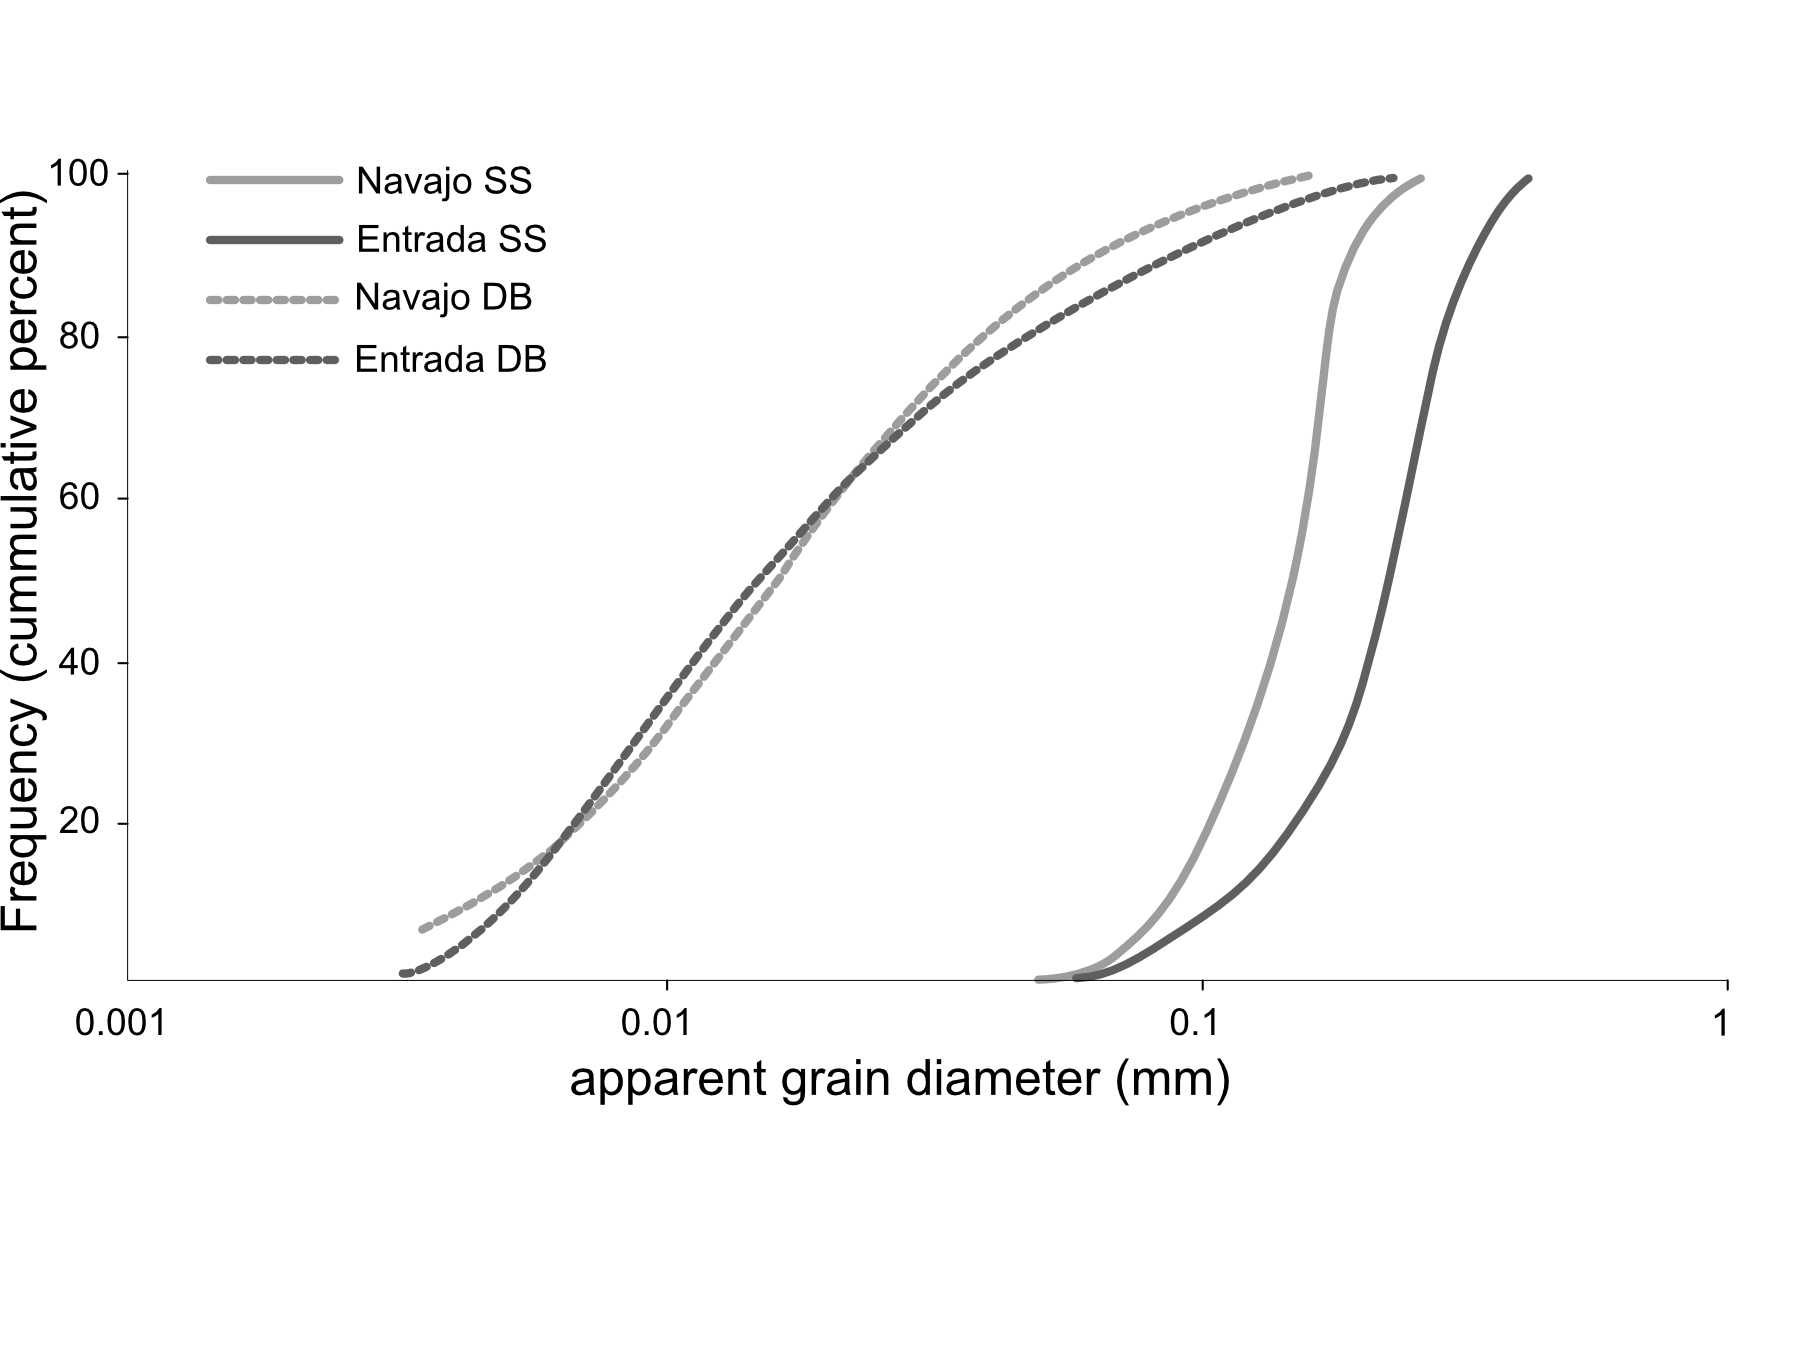
\includegraphics[width=\textwidth]{Grain_size_distribution}

	\caption{Grains size reduction of crushed grains within deformation bands relative to the underformed sandstone units, the Navajo and Entrada sanstones. (figure adapted from Aydin, 1978)}
	\label{grain_size}
\end{figure} 


\begin{figure}[h]
	\centering

		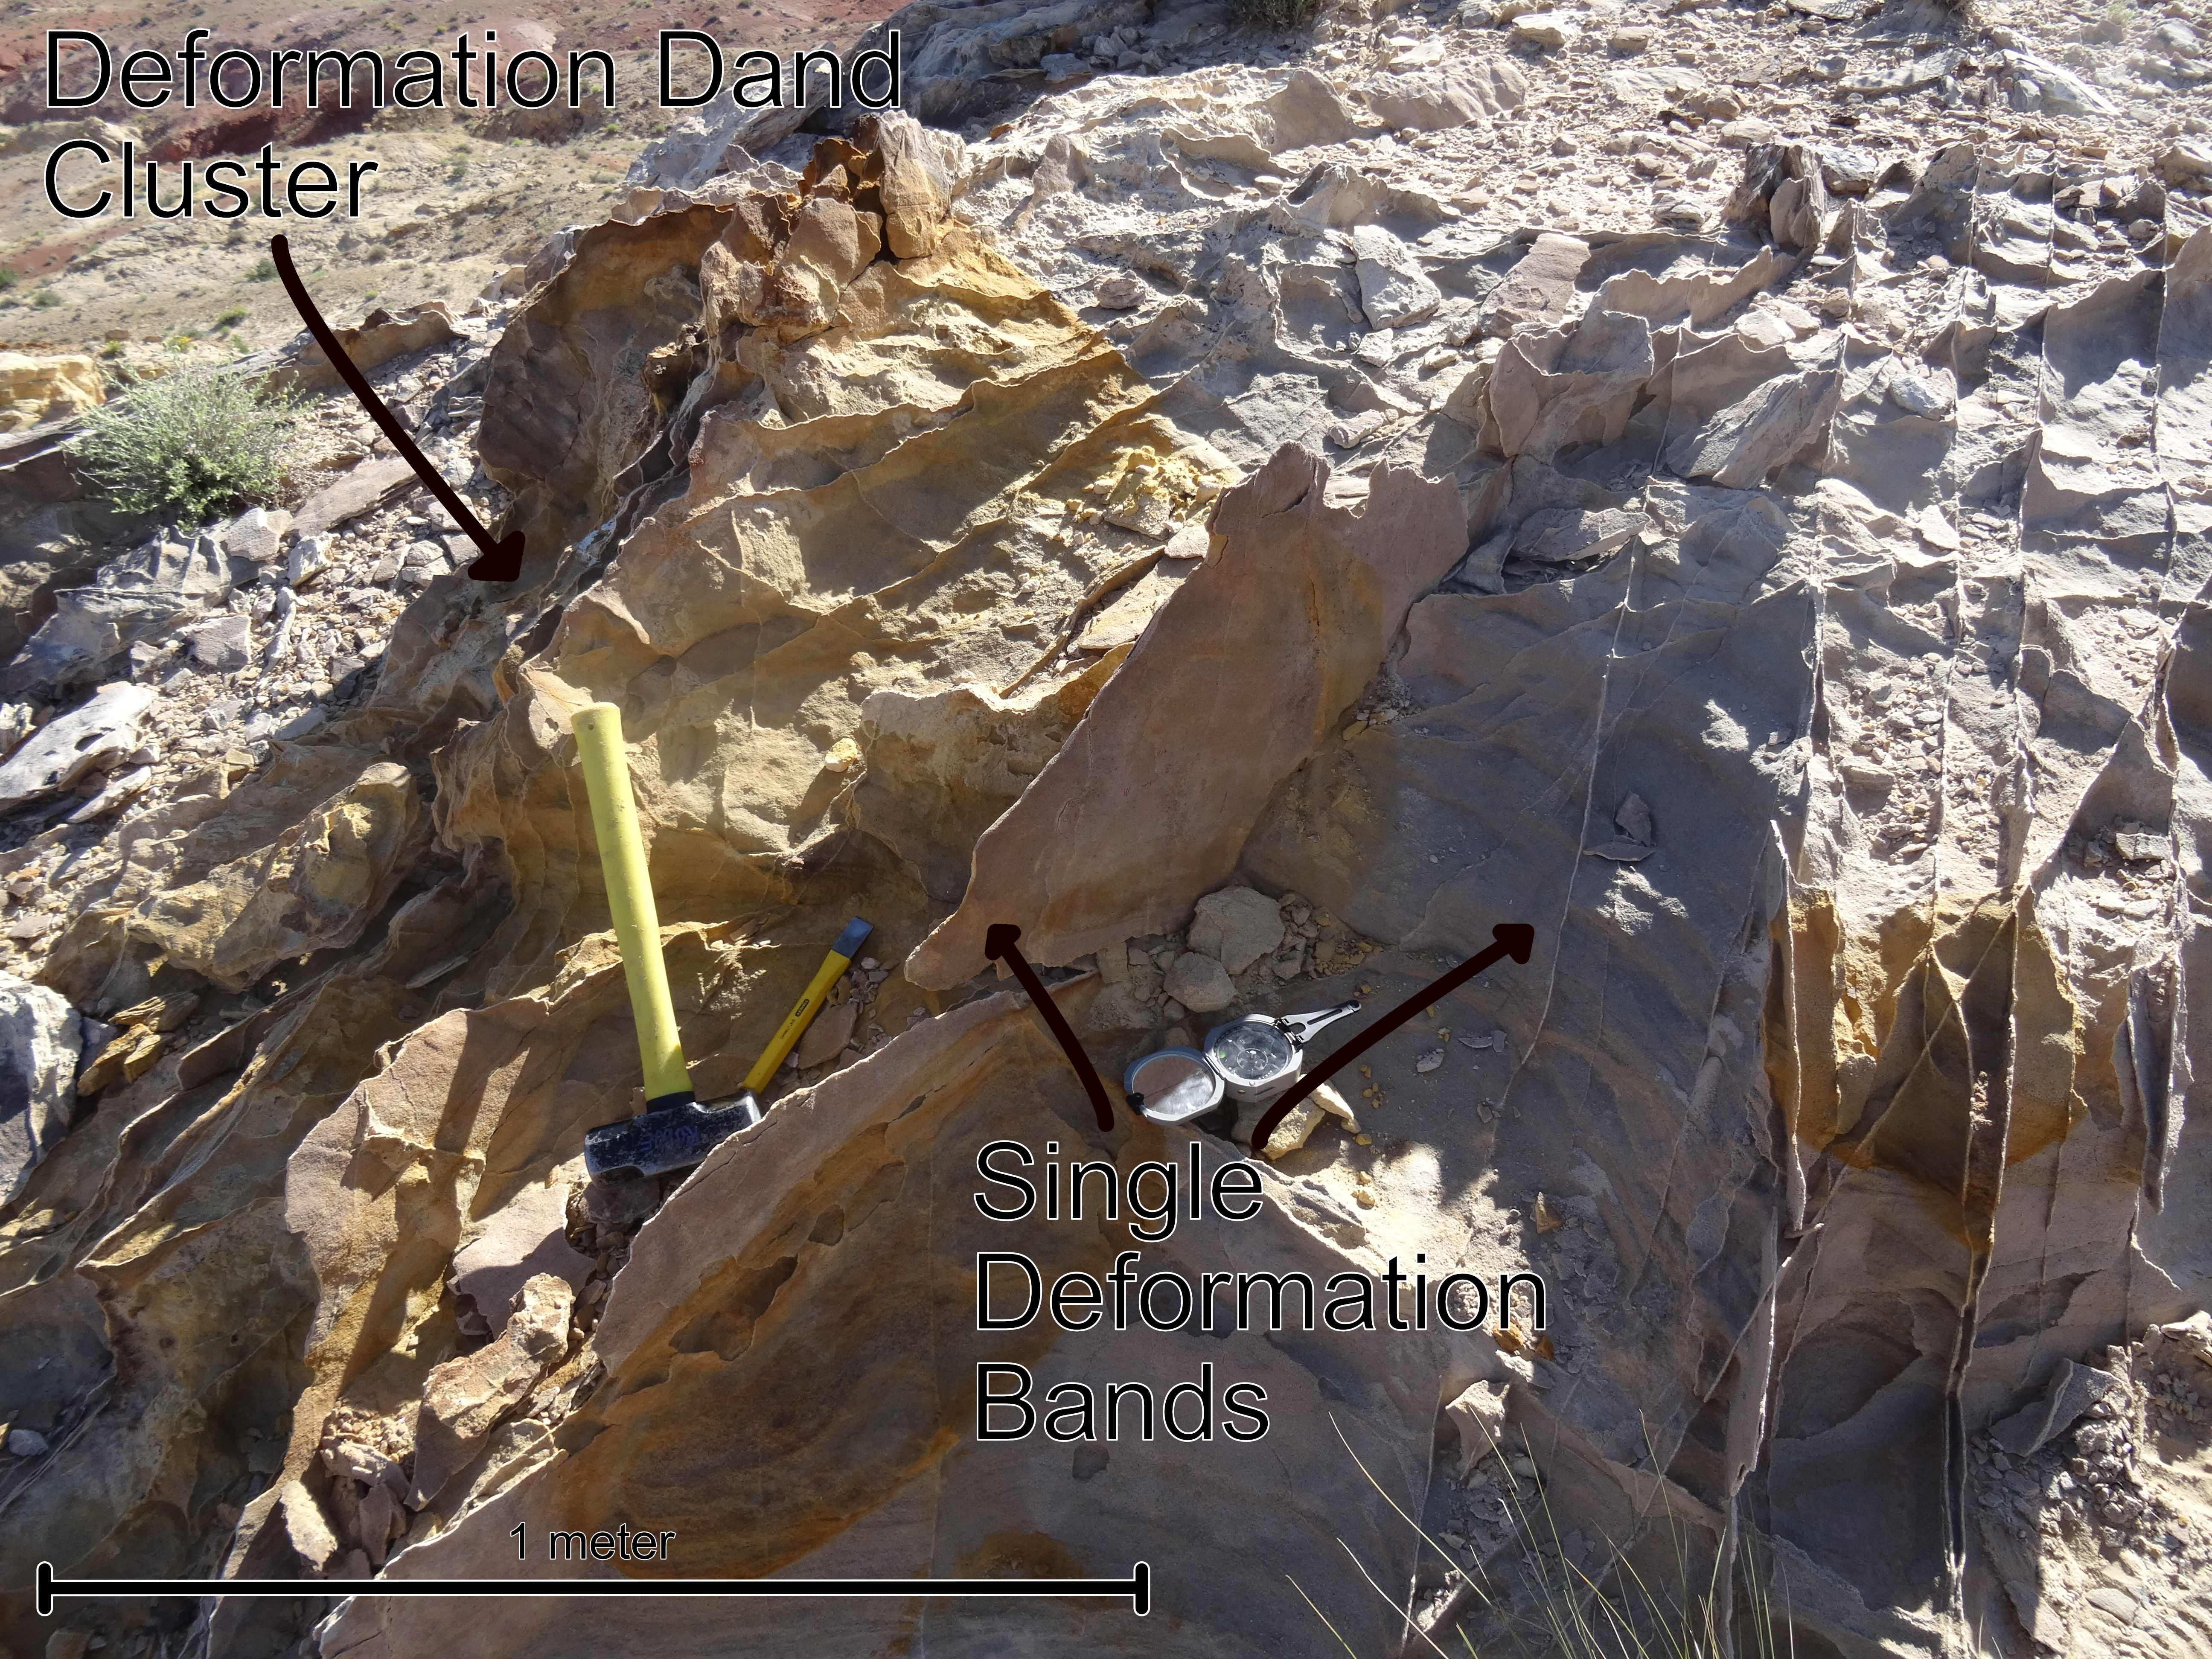
\includegraphics[width=\textwidth]{Defomation_Bands}

	\caption{Example of single deformation bands protruding out of outcrop. A small deformation band cluster is also visible in the background.}
	\label{deformation_band}
\end{figure} 

Deformation band clusters contain groups, or clusters, of nearly co-planar, mutually cross-cutting individual bands. The clusters are dense networks of anastamozing deformation bands. The clusters range in thickness from a few millimetres to tens of centimetres in width, often outcropping as slabs up to meters in height.  Clusters commonly form in upright conjugate pairs.

Deformation bands clusters have well defined edges. Given differential weathering, particularly characteristic for the Goblin Valley area, deformation bands form large meter-scale slabs. The exposed edges of deformation band clusters have distinctly corrugated and "lumpy" morphology (see figure \ref{DBC}-left). The corrugation is better defined that in individual deformation bands. The dip parallel rake of the corrugations is in general agreement with the normal, dip-slip, local kinematics. As is the case for individual deformation bands, edges of the deformation band clusters are always coated with a cohesive, single grain-thick layer of sand grains from the host sandstone. There is a clear directional asymmetry along the direction of shear whereby steep faces are in the direction of shear offset and shallowed faces are in the opposite directions (see figure \ref{DBC}). The asymmetry on the hanging-wall edges of the slabs is inverted on the foot-wall edges likely indicating an association with the overall kinematics of the clusters. Texture related to deformation band clusters are poorly captured in thin section because the size of any structural components exceeds the practical size of sections.


\subsubsection{Joints}

Subvertical joints sets are a common feature of every locality. Joint sets are best defined in the upper Navajo units and lower Carmel limestone pavements. The abundance of joints increases near faults. Joints surface can be very large- effectively defining cliff faces 10's or even 100's of meters in size. Joints are better defined in the Navajo and Carmel Unit than in the entrada. While spacing between joint in the Carmel pavements is tight (on the order of ~10 cm), the spacing in the Navajo appears to be much larger (~ 1 m or more). Joint surfaces are notably smoother than deformation bands, but rougher than slip surfaces. Salient morphological features on joint surfaces are the plumose structures relict from fracture growth and fabrics  aligned with cross-bedding horizons.

 \begin{figure}[H]
	\centering
	\begin{subfigure}[b]{0.4\textwidth}
		\includegraphics[width=\textwidth]{DBC_edge}
	\end{subfigure}
	~
	\begin{subfigure}[b]{0.4\textwidth}
		\includegraphics[width=\textwidth]{DBC_X}
	\end{subfigure}
	\caption{Left: Example of the edge of a deformation bands cluster at Molly's Castle. Note the "lumpy" morphology and an clear vertical directional asymmetry. Right: Cross-sectional view of a deformation band cluster with tens of centimeters of shear offset. It is unclear weather there is a through going slip surface localizing displacement. It is , however, definitely not on the edge of the cluster.}
	\label{DBC}
\end{figure}		


\subsection{Slip Surfaces}

Slip surfaces in the Navajo and Entrada sandstones are most readily identifiable by their relatively planar and polished morphology with a reflective or even vitreous polish. Striations and grooves on the slip surfaces mark the direction of slip. In cross-sectional exposure, slip surfaces are discrete, through-going and smooth relative to their zero-displacement counterparts. A sharp interface, separated by a sub-mm thick layer of incohesive white powder bounded by two vitreous surfaces. Thin milky white layers, less than a few centimetres in thickness, typically flank slip surfaces. These are in turn, within dense network deformation bands. The slip surfaces often cross-cut or bound deformation band clusters and the deformation bands within them. Perpendicular profiles are notably more sinuous than slip parallel profiles. Slip surfaces are incohesive, and readily form a parting surface.(see figure – figure similar to that in Jamies notes)

Slip surfaces are only preserved in the Navajo and Entrada Sandstones. For example, in spite of good exposures in prospecting pits and careful inspection of the slip zone, Navajo-Carmel contact at the Chimney Rock fault array does have preserved slip surfaces in the Carmel Unit. It is unclear whether this indicates that the Carmel units is more susceptible to erosion and/or alteration; or if a polished finish is only a feature of the quartzite sandstones.

 \begin{figure}[h]
	\centering
		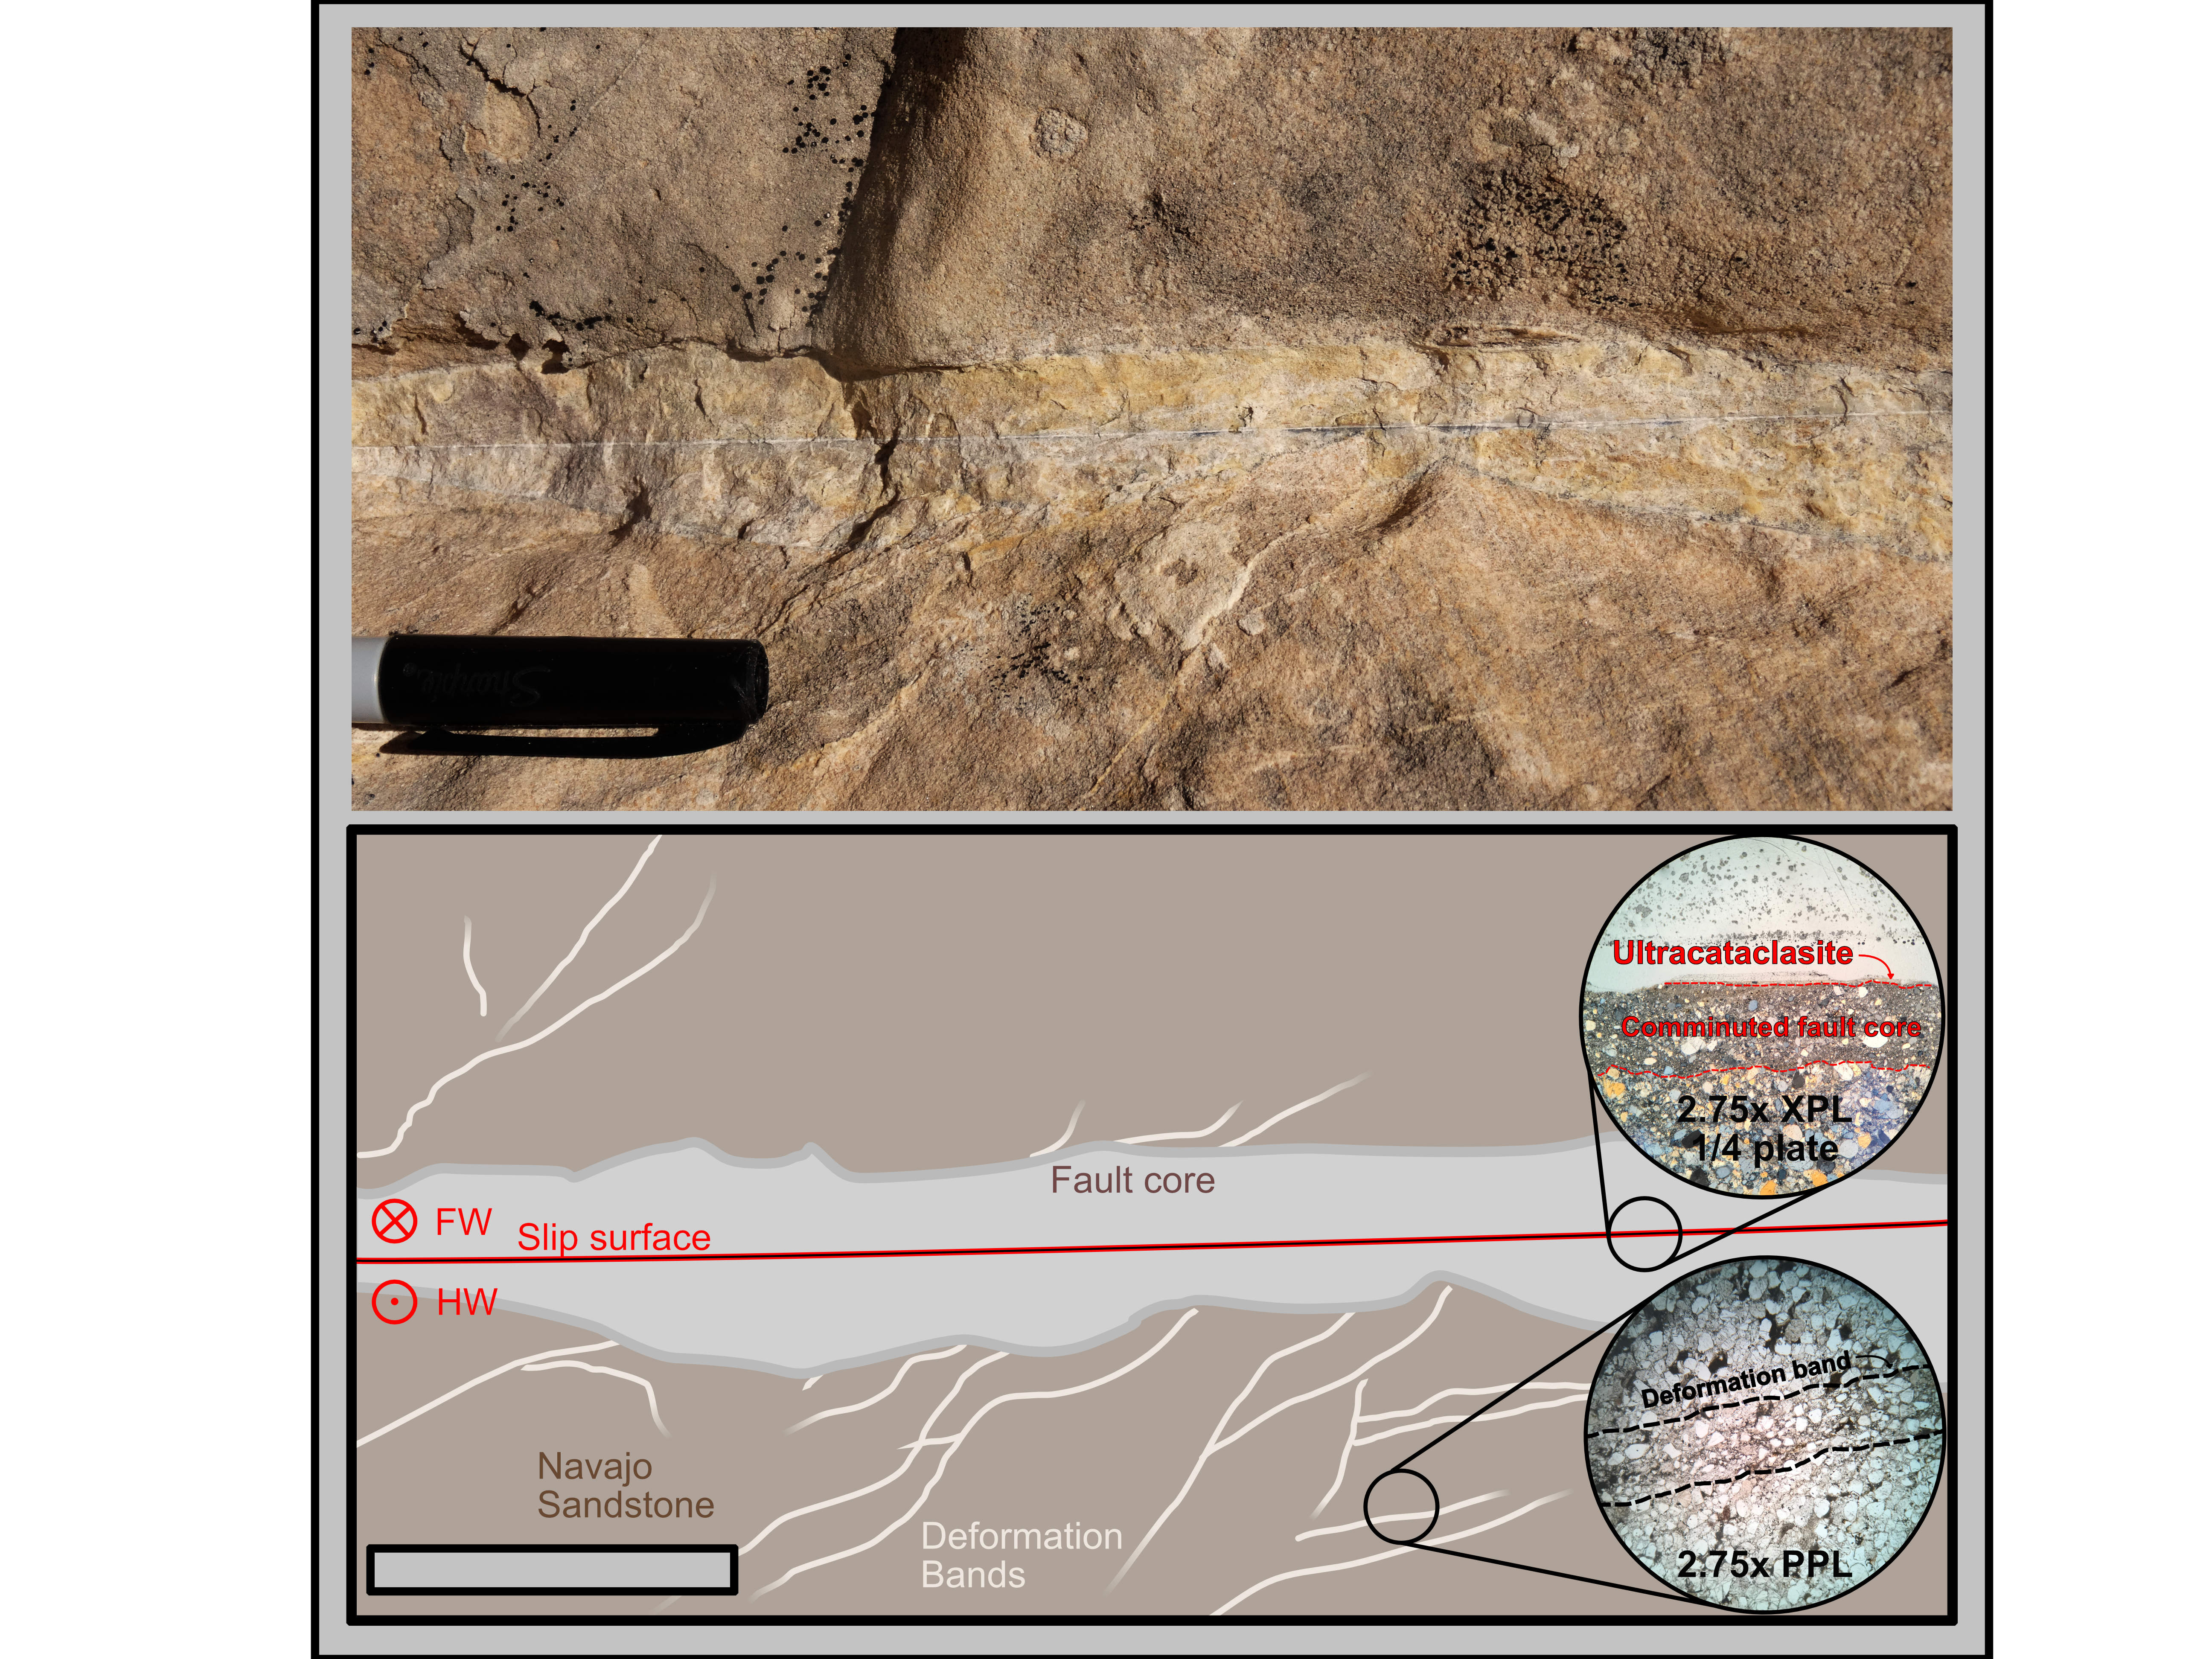
\includegraphics[width=1 \textwidth]{Fault_architecture_zoom}
	\caption{Top: Example of representative meso-structure of faults in the Navajo sandstone. Bottom: Cartoon of the representative meso-structure with slip surface (red), fault core (grey), deformation bands (pale beige) and intact host sand stone (brown). Upper half is the footwall; lower half is the hanging wall. Exposure is slip perpendicular. Representative thin sections show (not in situ) show the bottom half of the fault core (top) and deformation band (bottom). The section through the slip surface shows the microstructural architecture of slip surfaces with a very fine layer (barely visible) of ultracataclasite and a bounding comminuted layer. Note that this section is still well within the fault core. The section through the deformation bands shows the gradational reduction in grain size (outlined by black dashed line).}
	\label{DBC}
\end{figure}

	Thin section observations reveal a layered micro-structural architecture of the faults rock locally bounding slip surfaces. The following succession, ordered according to distance from the slip surface is typical for slip surfaces in sand stone:  1) a very fine grained ultracataclatic layer, 2) a broader cataclasite layer (sometimes absent) and 3) a deformation band zone, the density of which gradually decreases into 4) the relatively intact protolith with disparate deformation bands.

%In spite of careful preparation using epoxy, thin sections all parted at the slip surface interfaces. Moreover, samples only recording one side of the slip surfaces only partially preserved the edge of the slip surface.

	The ultacataclasite is continous, nearly always bounds the slip surface, and ranges from sub-milimeter to 2 milimeters in thickness. Texturally, the layer texturally overprints and cross-cuts all other layers. From visual assessment, the grain size distribution has a steep but continuous (no clast/matrix distinction) fall off with most grains being unresolvable at 400 fold magnification. Larger grains do not exceed 10's of micron - significantly smaller than protolithic intact grains which are on the order of 100's of micron. Grains have a large diversity in angularity ranging from sub-rounded to angular. We were unable to find fragmented counterpart within the ultracataclasite. This is indicative that the layer was likely fluidized \cite{otsuki2003fluidization}. There are patially offset survivor grains which could be interpreted as fragmented counterparts, however, these results from shear offset of fractures through-going the entire unltacataclastic layer. These fractures and grains they partially offset are instead indicative of cycling between healing and brittle failure postdating the formation of the fluidized ultracataclastic layer. Ultracataclasite layers preserve a faint, potentially compositional, foliation oblique to the fault. Interpreted as S-type foliations, the kinemtics from the flow banding are consistent with sense of shear of grains protruding into the utracataclasite and partially sheared off. Previous work has shown no notable change in relative abundance of major elements, silicon, calcium, potassium and sodiu, of the undeformed sandstones  \cite{aydin1977faulting}. We do however observe an increase in concentration in opaque oxides near the slip surface.	

	
	Scattered Electron Microscopy (SEM) reveals 

	A sharp, irregular and discontinuous interface juxtaposes the cataclastic layer to the ultracataclasite. The interface is characterized by a distinct difference in grain size and spatial arrangement. Past this transition, grains are larger and sometimes preserve damaged but intact sedimentary textures from the sandstone.

	The interface between the ultracataclasite and the cataclasite is more irregular then the slip surface. The irregularity is broadly associated with the following two distinct length scales: the grain scale and the 'scaloping' length scale (see figure \ref{microstructural_wear}. Grains at the interface are typically truncated such that their tops are completely flattened. The transition towards flattened grains is well captured at various different stages by instances where grains protruding into the ultracataclasite are still intact. ordered from least damaged to most damaged, we see the following: 1) grains that protrude into the ultracatclasite with little to no damage Other grains we evidence of healed internal cracks, 2) grains with various stages of mirco-cracking and fractures, with fracture orientations roughly parallel to the slip  and with some very small shear offset and, sometimes, rotation and 3) fully cracked grain with the fragmented counterpart rotated along slip or completely missing missing. While most of the fractures are only intra-granular, some fractures can readily be projected into neighbouring grain. 
	
	A larger milimeter scale geometry can be traced from linking fractures. Both ends of the fractures abut in the ultracataclastic layer with shallow obliquity ($~15^o$), such that the crack follows an arcuate path with an overall 'scalloped geometry'. The occurrence of these fractures seem to be anticorellated with the thickness of the ultracataclasite. Again, this geometry is recorded at various stages ranging from the alignements of multiple fractures within the catacla


\begin{figure}
	\centering

		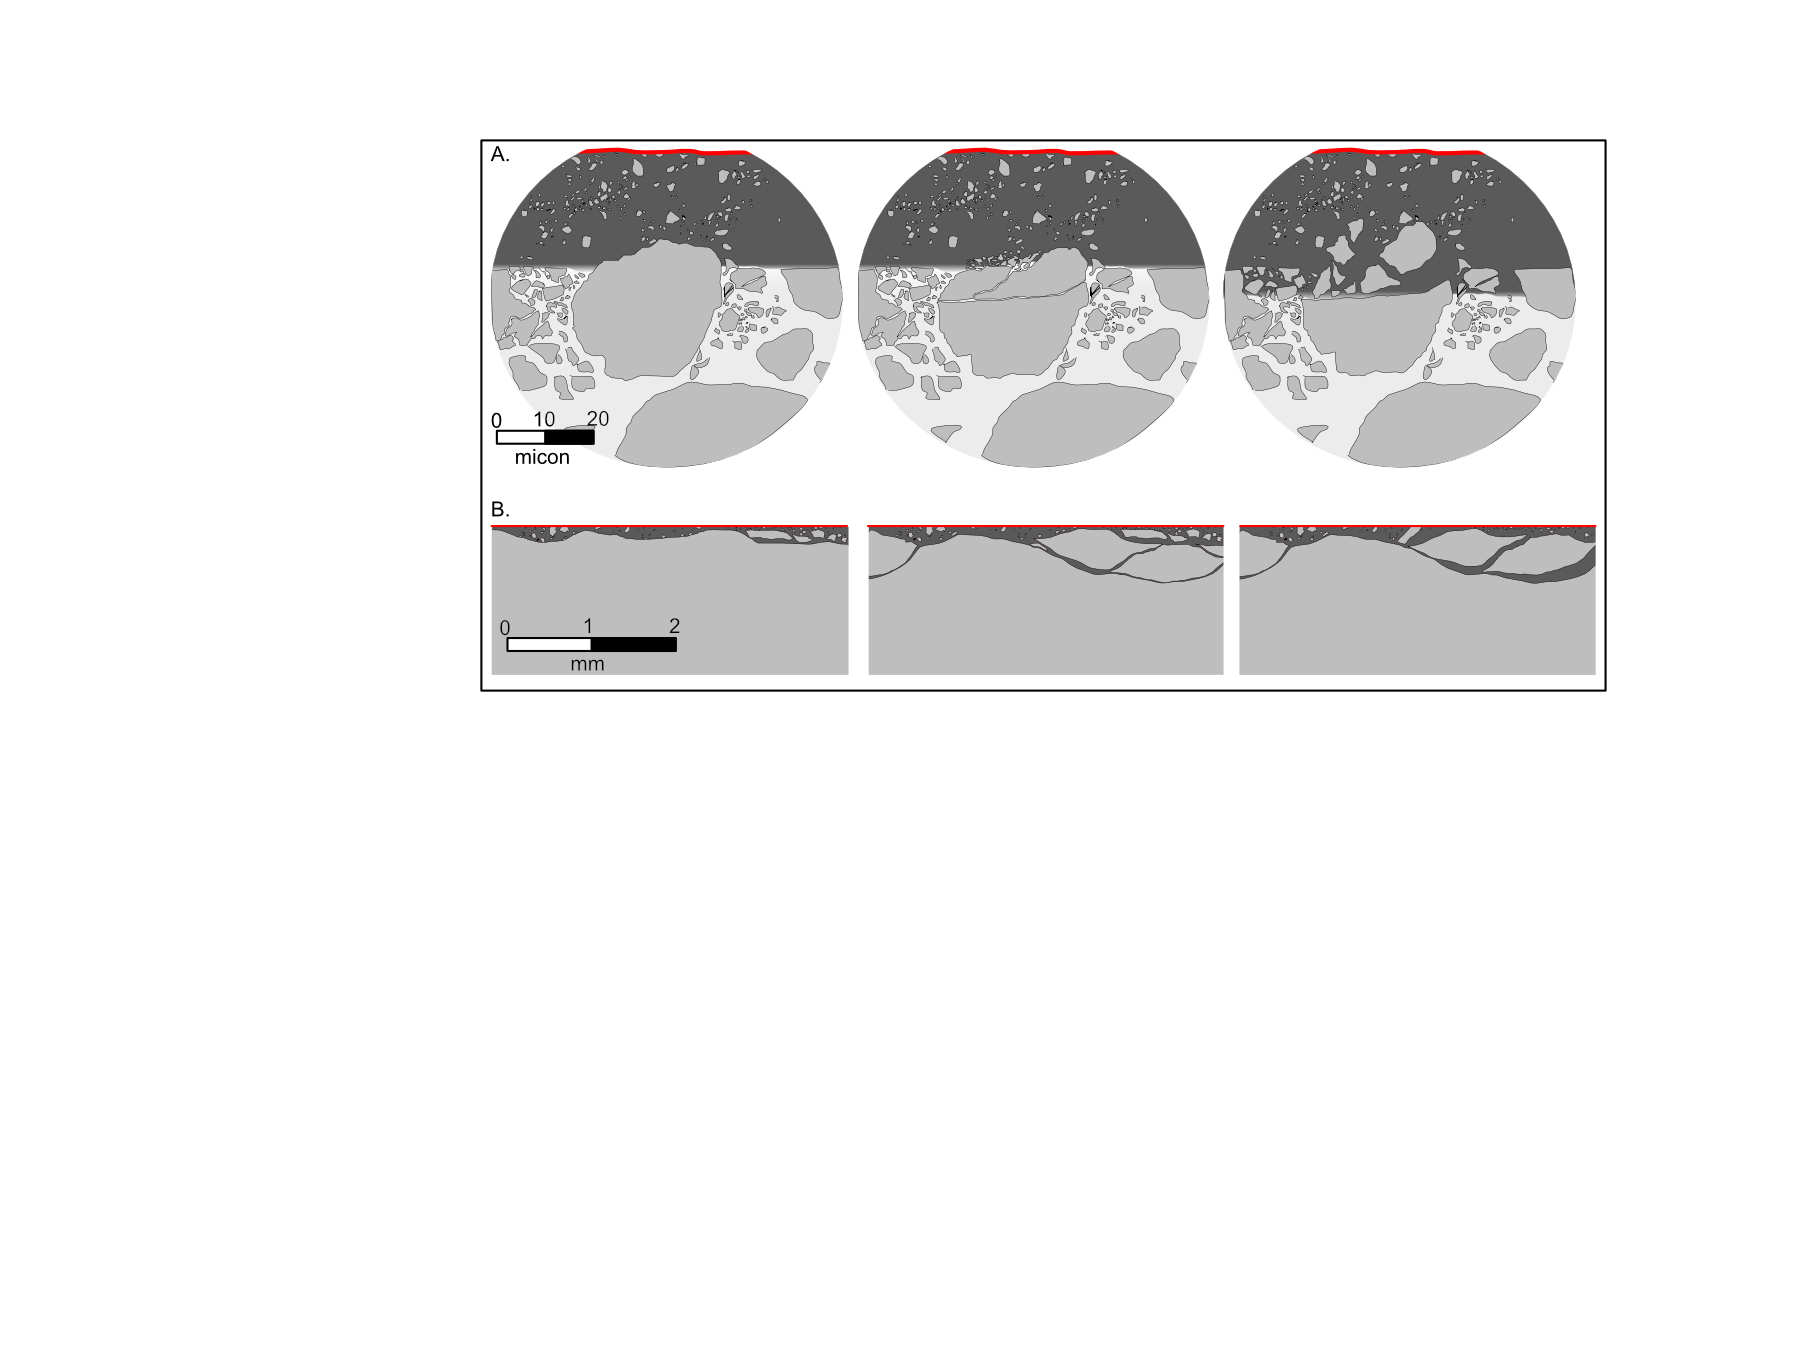
\includegraphics[width=\textwidth]{microstructural_wear}
		\caption{Schematic example of the interface between the cataclastic host and the fluidized unltracataclasite layer at two distinct length scales. A. at the length scale of ten's of microns grains, the shape of the interface is  }
	\label{microstructural_wear}
\end{figure}	

\begin{figure}
	\centering
    \includegraphics[width=1\textwidth]{PSS}
	
	\caption{Example of a slip surface interpreted as a principle slip surface with around 20 meters of displacement at Big Hole Fault}
	\label{PSS}
\end{figure}
	
	In contrast to the ultracataclasite, the original grain geometry is sometimes still discernible in the cataclasite. Grains size within the cataclasite layer is spatially variable with bands or lens' of larger grains separated by finer, more angular grains. These  layers are texturally similar in overall geometry to deformation bands have much smaller grains.

	This cataclastic layer thickness is highly variable. It typically ranges from millimetres to centimetres. Variability is directly associated with splay features which intensify mechanical damage around the fault. Its thickness on either side of the slip surface is often highly asymmetric. The layer is not always present.   When it is absent, the fault, still bounded by a thin ultracataclasite, directly transitions into the intact host. 
	
	For certain faults, dark oxide filled fractures up to a few centimetres in length abut steeply into the slip surface and over-print other fault-related textural features. These are characteristically consistent with dynamics tensile cracks. If this interpretation is correct, they would indicative of seismic rupture velocities.

	The evolution of slip surfaces with displacement is qualitatively apparent. Faults with small displacements (centimetres of offset) are distinctly different than larger displacement faults (meters of offset). They are 1) visibly more sinuous, 2) laterally discontinuous, 3) less polished, instead, having a dull lustre, and 4) not bounded by well-defined gouge or cataclasites layers bounding the slip surface visible in the field. The minimum observed offset across slip surfaces was approximately 0.5 cm. It is unclear whether this lower bound is a mechanical transition between deformation with deformation bands and slip on a discrete slip surface.

\begin{figure}
	\centering
	\begin{subfigure}[b]{0.4\textwidth}
		\includegraphics[width=\textwidth]{two_slip_surfaces}
	\end{subfigure}
	~
	\begin{subfigure}[b]{0.4\textwidth}
		\includegraphics[width=\textwidth]{Concentric}
	\end{subfigure}
	\caption{Left: Example of at least two distinct polished slip surfaces on the same fault structure. Right: Example of concentric pattern on cross-sectional view a fault}
	\label{many_surf}
\end{figure}	

\begin{figure}
	\centering
    \includegraphics[width=1\textwidth]{PSS}
	
	\caption{Example of a slip surface interpreted as a principle slip surface with around 20 meters of displacement at Big Hole Fault}
	\label{PSS}
\end{figure}

Our observations suggest that a single surface does not always accommodate the bulk of  the fault offset. Instead, fault zones often have many slip surfaces, sheared joints and splays which partition offset. 

Certain slip surfaces do accommodate the overwhelming majority of fault offset-- displacement accommodated by smaller neighbouring discontinuous slip surfaces is minimal (Shipton, XXX). Based on observations from previous workers and those made in this study where larger displacement slip surfaces are unambiguously identifiable, we generalized the characteristics of large offset slip surfaces for the Navajo and Entrada Sanstones as follows:

\begin{itemize}
	
	\item \textit{Large displacement slip surfaces are more discrete and planar}.
	
	\item \textit{Larger displacement slip surfaces are not cross-cut by deformation bands or more sinuous and discontinuous slip surfaces}
	
	\item \textit{large displacement slip surfaces are nearly cohesionless and forming easy parting surfaces}
	
	\item \textit{Large displacement faults have a very vitreous finish};
	
	\item \textit{Large displacement slip surfaces are typically in the center of a damage zone}. 
	
\end{itemize}




\textbf{Damage is an inevitable consequence of displacement and the accompanying mismatch that accumulates. Damage at the field locations in this study is expressed as comminution (\textit{e.g.} cataclasite and gouge), fragmentation (\textit{e.g.} breccia, splay joints) and shear deformation (specifically deformation bands).}

In this study, we refer to \textit{fault rock} as rocks  associated with a fault (Snoke et al. 1998). The faults in our study area display a very diverse range in fault rock lithologies, ranging from fine-grained cataclasites to massive  bodies of breccias (up to meters of thickness). 

Fault rock consistently bounds slip surfaces--often asymmetrically. However, observations at the outcrop scale (10’s of meters) both along the strike and dip indicate that both the lithology and thickness of the fault rock are highly heterogeneous and are subject to large variability. These observations are consistent with more detailed fault architecture mapping conducted by Shipton et el., 2002.  

We do not observe a clear and tractable relation between fault slip surface displacement and faults rock thickness. This is big part a result of difficulties in defining a clear fault rock thickness criterion which well encapsulates the variety of faults rocks -- a challenge well highlighted in  (Shipton et al., 2006).

* this stuff is left over's from  editing and moving things around

Healed Gouges

-	the spot at big hole

-	iron wash (powder between the surface)

-	micro-structure

-	prospecting pit

-	typically on thinned sections of the fault rock (near the slip surface)
Cataclasites ….

-	big hole sample with slip surfaces on both sides of the cataclasite

-	micro-structure
-
Breccias…

-	thick sections  of the 
Breccias occur lenses which range from cm’s to meters in thickness. Breccia clasts are typically poorly sorted and can be very coarse with clast up to ~10 cm in diameter. Clasts show indications for multiple generations of brecciation.


Thin Quarts lens
-	iron wash


Systematic associations between fault rock and fault structure exist. For instance, Davatzes et al., 2002 reports of a systematic association between the fault rock lithology and the orientation of the fault set. Namely, the orthorhombic fault set striking WNW has systematic association with fragmentation—fault breccias; conversely the ENE fault set rather has slip surfaces cutting through deformation band clusters (see figure \ref{fig:DavatzesFR}). This relation was speculated to be the result of contrasting genetic mechanism. The WNW set is the result of the reactivation of regional joints. In contrast the ENE fault set is the the result of clustering and anastamosing deformation bands acting as a catalysing agent to the formation of a faults.
In this study, we observe clear instance of lithological contacts being associated with brecciation (photo at iron wash where the top of the Navajo is brecciated and quickly reverts to a single fault strand. More over, large breccia bodies are clearly related to points where faults are cross-cutting each other at high obliquity as is often the case at the Chimney Rock fault array and 

Complicating factors:

Associations between brecciation and lithological contacts…

Associations between brecciation and cross cutting faults…

For an extensive review and description of the faults in the Navajo and Entrada sand stones refer to Aydin’s thesis. 


\subsection{Interpretation of field observations and roughness measurements}

Cross-cutting relationships reported bot in this study and in previous work on faults in the Navajo and Entrada units of the San-Rafael swell are particularly informative. Large displacement slip surfaces are not cross cut by deformation bands and more sinuous slip surfaces. However, large displacement slip surfaces do cross-cut clusters of deformation bands and more sinuous slip surfaces. This relationship is indicative of a clear evolution of the fault architecture by 1) localizing displacement and 2) smoothing out slip surfaces. 

Faults zones with larger offset are associated with larger damage zones and more slip surfaces. This is particularly telling fact when with the observation that small displacement slip surface do not cross cut larger displacement slip surfaces. 

The cross cutting relationship implies that either slip either smaller less continuous slip surfaces pre-date the onset of the larger offset slip surface or that the they splay off of it. However, we can reject the former as a possible mechanism as it does not account for the increased density of slip surfaces on larger offset fault zones.  This implies that they either form directly from the stress heterogeneities induced by the roughness of larger displacement slip surfaces. 

Slip surfaces pre-dating large The former case  stress heterogeneities from active slip surfaces induced by fault roughness.

%Observations from this study do not necessarily agree with this paradigm. deformation bands active after the onset of a stable slip surface \textit{have} been observed at Big Hole (Shipton and Cowie, 2003). Onset of late deformation bands may reconcile our observations with the existing paradigm for fault development in high porosity sandstones. We intend to explore the surface roughness of the edge of deformation band clusters. In a sense, these surfaces could represent a 'primordial roughness'.%

%At some locations, take for instance the Blueberry Fault in the Chimney Rock Fault Array, deformations bands seems to be the overwhelming mechanism to accommodate off-fault damage. When considering issues of fault mismatch related to roughness and consecutive displacement, deformation bands may be an effective mechanism to accommodate inelastic fault perpendicular deformation.%

faults are smoother than joints or deformation bands

At the grains scale, grains are truncated, not `plucked'.

more linear fault traces where not offset by wavier fault traces

%Damage is an inevitable consequence of displacement and the accompanying mismatch that accumulates. Damage at the field locations in this study is expressed as comminution (\textit{e.g.} cataclasite and gouge), fragmentation (\textit{e.g.} breccia, splay joints) and shear deformation (specifically deformation bands).

\textbf{The textural transition between the ultracataclasite and the cataclasite is best explained  by dynamic grain size reduction and wear at the slip surface interface producing ultracataclasite which overprint more diffuse off-fault grain size reduction through grain crushing and deformation band production.} 

	
\section{Geometric analysis}		

\subsection{Method}

Previous efforts to correlate fault roughness to displacement where frustrated by limited cliff-size exposure and bad displacemement constrains, fundamental to the quantitative analysis of the roughness data (i.e. \cite{sagy2007evolution, brodsky2011faults, candela2012roughness}). Field methods in this study correspondingly prioritize 1) slip surface quality 2) good displacement constraints 3) the number of faults scanned. Note that we do not necessary prioritize large exposure size as has been done in previous work.

We collected high precision, high density measurements with optical scanners in the field and, later, in laboratory on collected hand samples. Every scan was associated with a constraint on displacement. Moreover, we also recorded the time of day, location, quality of the slip surface, strike and dip of the fault slip surface, slickenline rake, and both plan and cross-sectional photographs. When permitted by outcrop exposure, we recorded an estimate of the fault rock thickness. See appendix for the tabulation of this data. Together, all these measurements and observations should provide the necessary data to robustly explain and quantify the processes through which faults mature.

	\subsubsection{Scan Data Acquisition}

A scan of a fault slip surface discretizes it into a \textit{point cloud}, a series of $x$, $y$ and $z$ coordinates. We measure slip surface roughness by analysing these point clouds scans. Specifically, we average the slip parallel and perpendicular spectral and statistical properties across hundreds of profiles. To ensure the fractal scaling is well-captured by the point cloud data, we use the following three scanning instruments capturing various scales of observations: a New View 8000 structure image analyzer (Zygo Corporation), a NextEngine desktop laser scanner and a BLAH BLAH LiDAr.  Together, these instruments offer the potential to resolve fault slip surface geometry with high accuracy and precision at over nine decades of length scale.

*make a map of each areas with the location of every scan encoded with different symbols*

A light detection and ranging instrument was used to resolve length-scales ranging from meters down to millimetres, (i.e. LiDAR). LiDar has been used in many previous studies of fault roughness as it is easily deployable in the field and provides rapid means to collet very large point cloud data set. However, its use is limiting as it requires exceptionally good and, accordingly, rare exposure of fault surfaces that are large enough and fresh enough to not have been degraded by erosion. In this study, we report 5 ??? Lidar Scans (see figure).

The bulk of \textit{in situ} field measurements were made at intermediate length-scales ranging from centimetres down to hundreds of microns with the NextEngine desktop 3D laser scanner. The NextEngine laser scanner has a working distance of 13 to 57 $cm$. Maximum accuracy, point cloud density and resolution are all broadly function of the working distance. In this study nearly all scan where measure at the optimal minimum working distance (15 cm). Accordingly, point clouds measured this study are expected to have an accuracy of 0.01 $cm$ and a point density of 41 540  $points/cm^2$. surface both to industrial-grade laser scanner as reference. The scanner is not exactly built to be field ready. It requires a power source, low light conditions, a stable surface to sit on, limited dust exposure and must be connected to a computer. Therefore, to use the scanner in the field, we connected both the laser scanner and laptop to a solar powered, \textit{Goalzero} battery. The scanner was encased and padded in a reinforced cardboard box cut such that the depth exactly corresponds to the optimal instrumental depth of field. The set up had the added advantage of being very portable, completely removing sunlight and limiting dust exposure. We report 45 scans using this field apparatus.

Finally, hand samples were collected and at McGill laboratories using white light interferometery. Slip surface samples are cut to be roughy 1 $cm^2$. We apply a 4 $nm$ platnmum coating. Point clouds where then produced using the New View 8000 structure image analyzer (Zygo Corporation). The instrument is an optical profilometer using a non-contact method, instead using a scanning white light source. The profilometer can capture surface geometry over length-scales ranging from millimetres down to hundreds of nanometres by using 2.5, 10 and 50 fold magnification objectives. Point point-clouds are relatively small, however it is possible to seamlessly stitch smaller scans together. Point clouds where benchmarked to a silicon carbide mirror reference. For the purpose of this study, all samples where scanned at 20 and 2.75 magnification objectives. Scans obtained at 20 fold magnification where stitched together to produce sections roughly 2 by 4 millimetres with over $10^7$ points. Scans obtained at the 2.75 fold magnification are typically on the order of the sample size and have $10^6$ points. The later length scale nicely bridges the interferometry and laser scanner spatial resolution. We report on 73 point clouds obtained with the white light profilometer.

\textbf{We assess the effect of erosion of slip surfaces by qualitatively comparing freshly parted slip surfaces with fault scarps with surfaces that have been exposed to the elements for a long time. Weathered scarps do preserve slip surfaces. However, these have a reddish-brown to dark tarnish and less vitreous lustres. Sections of the slip surface are plucked off. Severely weathered scarps develop a slip perpendicular fabric associated with conjugate fractures and deformation bands abutting into the slip surfaces. These surfaces where not scanned. From our field observation, it is clear that erosion has the effect of re-roughening the slip surfaces, especially at smaller scales. We can confidently attribute these re-roughening effects to erosion because they did not occur in freshly parted slip surfaces. The extent of weathering and erosion was noted and taken into account in post-processing stage on data analysis.}

	\subsubsection{Constraining displacement}

We associate every scan with displacement constraint. At The Chimney Rock Fault Array and Big Hole Fault, entire displacement and/or throw profiles have been measured during previous mapping campaigns (\cite{krantz1986orthorhombic, krantz1989orthorhombic, maerten2001digital, shipton2001damage}). For the Chimney Rock fault array, we use geospatial data obtained from Maerten (personal communications). At big hole we used maps in \cite{shipton2001damage} as reference. At Iron wash, Horse Creek and Molly’s Castle, Atilla Aydin’s mapping identified clear offset markers where available (\cite{aydin1977faulting}). For these field locations we use maps available in \cite{aydin1977faulting}. When necessary base maps for all field locations were digitized and georeferenced using satellite images. Maps where all used the field to streamline scan data acquisition. Displacement were estimated after the field campaign using GPS locations collected in the field. Additional measurements using basic tape measure and compass triangulation methods where also obtained in the field to obtain true faults slip surface displacement.  

Base maps only report stratigraphic throw or, in some cases, offset across fault zones. However, many slip surfaces, complex networks of deformation bands and sheared joints which partition offset across fault fault zone (see figure). We therefore make a distinction between \textit{offset} across an entire fault and \textit{displacement} across a single slip surface. Without good marker horizons and cross-sectional exposure, how stratigraphic offset is partitioned across slip surfaces is ambiguous. Offset across the entire fault zone therefore only serves as an upper-bound constraint on displacement across a single slip surface slip surface. For 60\% of point cloud measurements, this is the best available constraint on displacement. 

\begin{figure}[h]
	\centering

		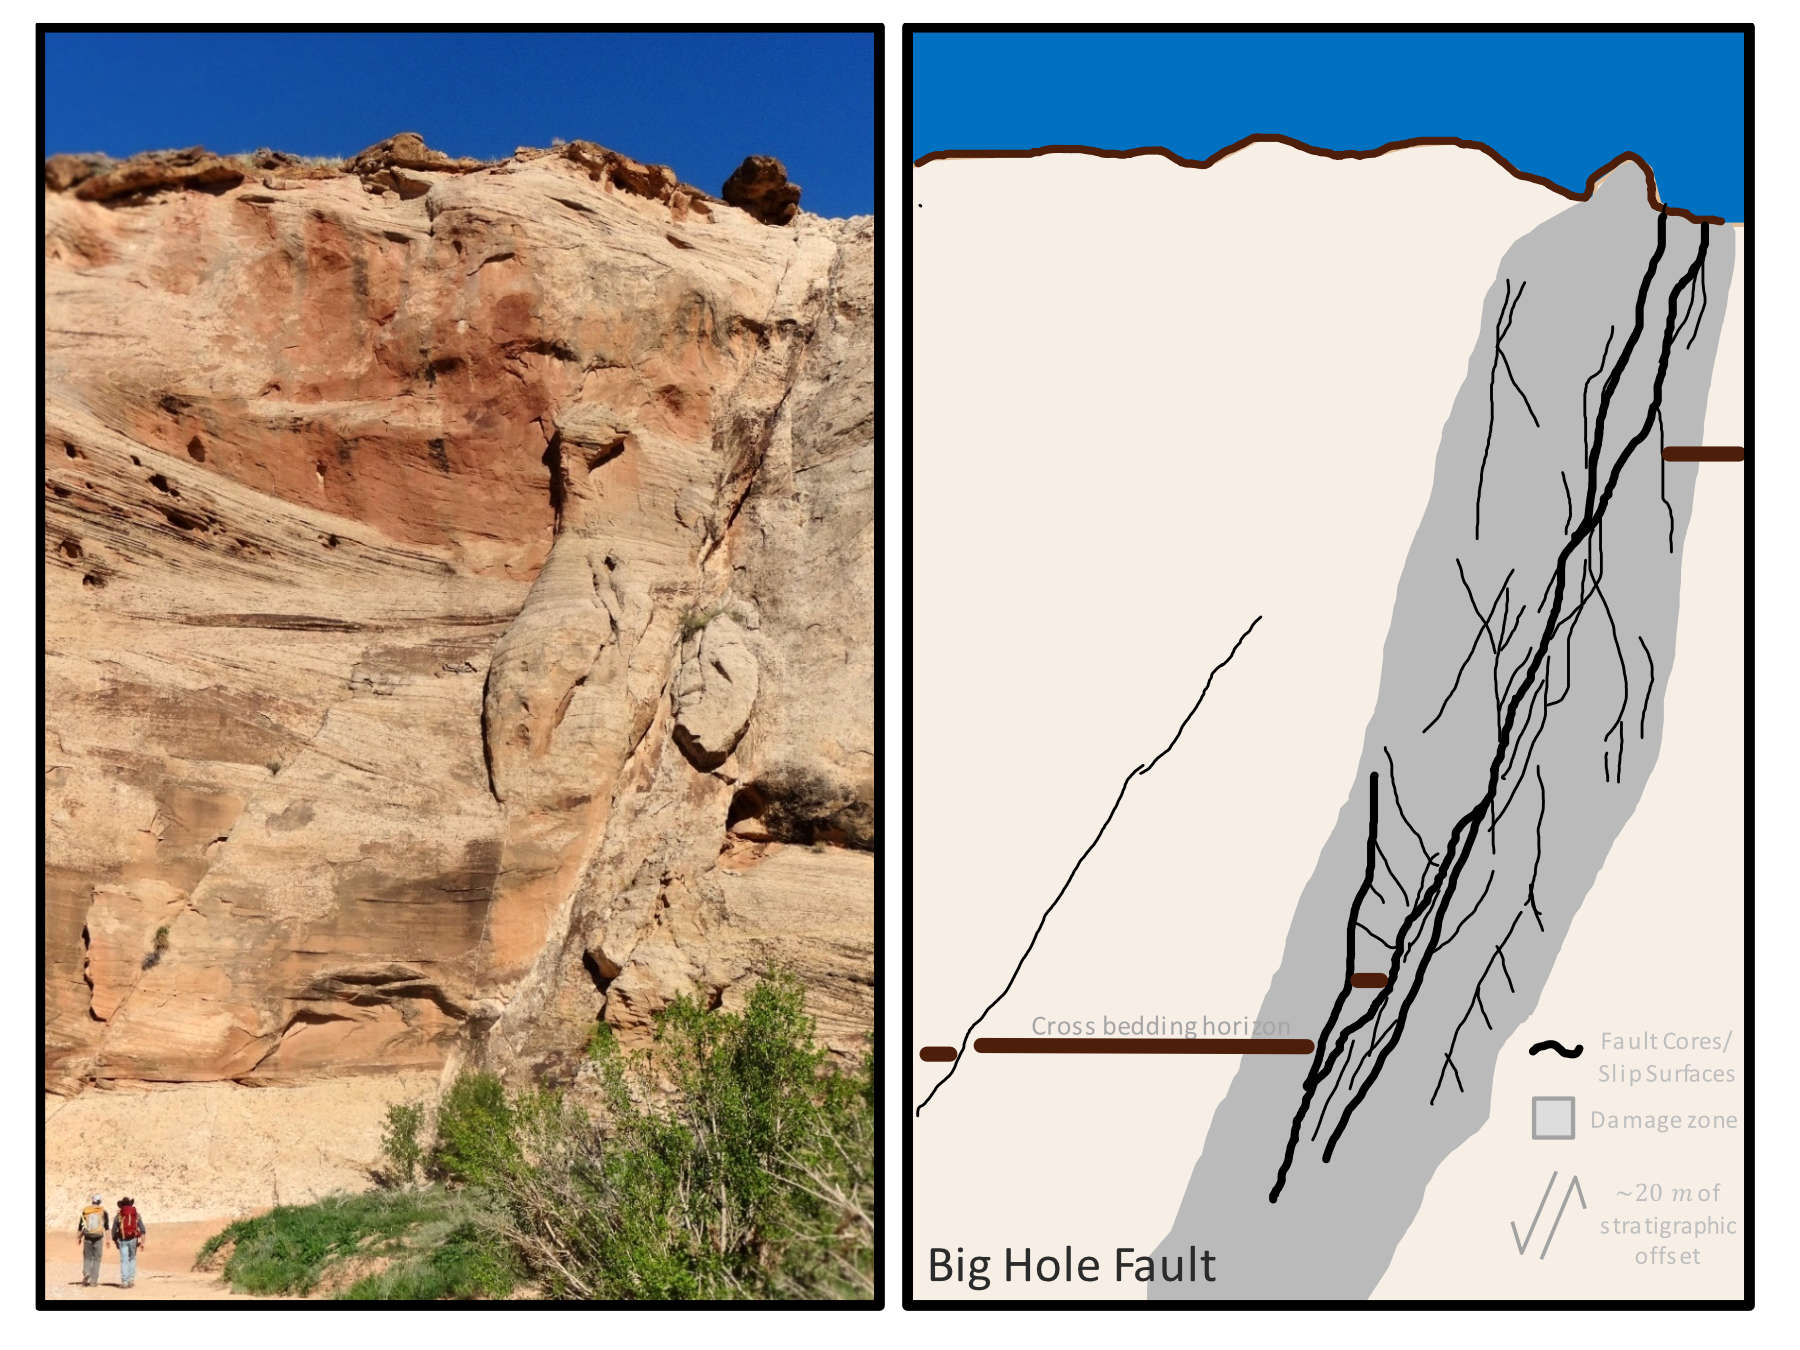
\includegraphics[width=\textwidth]{big_hole_cliff}

	\caption{At Big Hole fault, two large-scale continuous strands of the fault, both accommodating meters of displacement exemplify problem at a larger scale. Due to the ambiguity, Shipton and Cowie, 2003 report large uncertainty on the partitioning of stratigraphic offset across the two strand}
	\label{big_hole_cliff}
\end{figure}  

We were able to reconstruct exact displacement in the following specific cases: 1) if cross sectional exposure indicates only one slip surface; 2) If cross-sectional exposure is good enough to clearly indicate cutoff surface (lamella, cross-bedding or lithological contact); or 3) following \cite{chester1986implications} and, locally, \cite{shipton2001damage}, if it is unambiguous that there is a \textit{principle slip surface} accommodating the overwhelming majority of fault offset, i.e. it is continuous, it has a layer of fault rock and is unmistakably more linear and sharp than any other slip surface in the fault zone. 

Errors on displacement estimates are either reported directly for previous work when available. For Chimney rock, we report $1m$ precision based on high resolution GPS mapping by Maerten et al., 2001. For Big Hole, we report $5m$ precision based on total station surveying by Shipton et al., 2001. For our field measurements and those made by Aydin, 1977, we report conservative $10\%$ error on displacement estimates. 

	\subsubsection{Scan data Processing}

We use point cloud spatial statistics to characterize and quantify features of the topography that could record active surface processes on faults. We develloped a \textit{MatLab} work flow to entirely automate data processing from the raw \textit{.xyz} input fromat to the final statistical analysis:

\begin{enumerate}
	\item Preprocessing
	\begin{enumerate}
		\item manual inspection and removal of coarsest defects in built in scanner software
		\item export point cloud data to \textit{.xyz} data
		\item Import \textit{.xyz} data into \textit{Matlab}
		\item Very coarse Height field filter (standard deviation threshold)
		\item Rotate mean plane to horizontal
		\item Orient grid along slip direction (using power spectral analysis)
		\item re-grid to even point spacing
		\item Remove defects
		\begin{enumerate}
			\item Remove outliers in the height field (standard deviation threshold)
			\item Fractal model filter
			\item Remove re-gridding artefact 
		\end{enumerate}
	\end{enumerate}
	\item Processing
	\begin{enumerate}
		\item Statistical analysis
		\begin{enumerate}
			\item Scale-dependent \textit{RMS}
			\item Scale-dependent skewness
			\item Scale-dependent kurtosis
			\item Scale-dependent asymmetry
		\end{enumerate}
		\item Spectral Analysis
		\begin{enumerate}
			\item Fast Fourier Transform (FFT)
			\item Lomb-Scargle Periodogram
		\end{enumerate}
	\end{enumerate}
\end{enumerate}

\textcolor{red}{\textit{make into figure, include bypasses and other recent additions}}  
	 
	Before conducting a statistical analysis scan data must be pre-processed into a workable format. Scan data is a point cloud - a series of points with coordinates $x$, $y$ and $z$. Scans reported in this study typically have $10^6$ to $ 10^7$ points. In raw form, the point clouds are randomly oriented, noisy and still contain instrumental and physical artefacts. Physical artefacts include cracks, eroded sections, and vegetation; instrumental artefacts include noise, smoothing and scattering. All these features must be removed. The process of manual removal is labour intensive and infeasible for a data set of the scope presented in this study. I rather opt to automate this process. Only very large defects (defects that may substantially effect the quality of finding a true mean plane) are manually removed.

The surface must first be rotated such that the mean plane is horizontal and aligned along slip. Linear trends in the data induce unwanted high frequency signal in data and also affect the quality of interpolation in upcoming steps. Thus, $x$, $y$, $z$ data is rotated around the axis $\textbf{u}$ determined by the normalized cross product between the normal vector to the mean plane of the point cloud, $\textbf{n}$, and the unit vertical vector, $\textbf{n}_2$: 

$$ \textbf{u} = {\textbf{n}\times\textbf{n}_2}/{|{\textbf{n}\times\textbf{n}_2}|} $$

with the rotation,

$$ R = \cos\theta\textbf{I} + \sin\theta[\textbf{u}]_x+(1-\cos\theta)\textbf{u}\otimes\textbf{u},$$

were $[\textbf{u}]_x$ is the cross product matrix of $u$ and $\otimes$ is the tensor product and $\textbf{I}$ is the identity matrix. 

Fault surfaces are anisotropic \cite{lee1996structural}. The direction of slip is preserved in the anisotropy whereby the 'smoothest' direction is slip parallel and the 'roughest' direction is perpendicular to slip. The fault scan is rotated around the $z$ axis such that the direction of slip is parallel to the $x$ axis. The direction of slip is found by decimating raw data before performing spectral analysis along directions rotated by $1^o$ increments around the z-axis, iterating through the steps of regridding at each rotation. In this radial search, roughness is quantified as the integral of the log-weighted power spectrum over the entire bandwidth of the sampled surface. The direction in which the roughness attains a minimum value is then identified as the direction of slip and subsequently used to rotated the original point cloud. The data is then interpolated onto a grid using a linear interpolation algorithm. The point spacing of the grid is automatically defined by the point density over the areal extent of the data:

\begin{equation}
	\Delta x = N_{pts}/A
\end{equation}

Where $Delta x$ is the point spacing, $N_pts$ is the number of points and $A$ is the areal horizontal extent of the data. The later is determined using a convex hull over the $x-y$ projection of the point cloud. This treatment results in the point spacing of the grid to be roughly consistent with that of the original scan.

INCLUDE HISTOGRAMS FOR EACH FILTER

\textit{Defects} include all physical surface features that are clearly not associated any faulting process, \textit{e.g.} cracks, eroded patches, vegetation, etc.. Defects are idenetified and filtered out using combination of thresholding methods. These methods all involve identifying points or linear segments of points that are statistical outliers to the distribution characterizing the entire surface. 

The most aggressive filter implemented searches for outliers to the fractal model. The filter removes entire linear segments of points with abnormally high variance in the height field for the given scale of observation. For this implementation, I iterate over 10 filter segment length-scales. The length-scales are selected using a log spacing between the 10 points and the length of the entire surface. The threshold for segment removal is chosen to be four standard deviations from the mean  which accounts for $<0.1$ percent of a normal distribution. Note that, assuming a normal distribution of data for a given scale, the filter does not induce a systematic bias in the mean value, since the filtering is symmetric around the mean. However, surface features associated with a truly distinct mechanism of formation, in this case cracks and other defects that will typically have much higher variance, \textit{are} be removed. This general approach ensures that defects, regardless of their scale are identified and removed.

In some cases, abnormally flat sections are introduced into a surface height field during the interpolation of sparse points. Typically, interpolation on the edge on a non-convex set of points is subject to this effect. These artefacts are readily identified following calculation of the surface curvature data. In the log-transformed absolute value curvature field, these sections appear to be nearly or exactly zero. The filter rejects point with curvatures less than $10^{-25} m^-1$. These values are assumed to be the result of the linear interpolation scheme.

Finally, all scan are inspected to make sure that the pre-processing was successful. The workflow fails to properly process scans that have too many defects surface defects. This is because 1) the mean plane is skewed by surface defects and in turn affects identifications of outliers in the height-field; and 2) the distinction between the fault surface and outliers becomes less distinct in the fractal model. These scans were manually cleaned and oriented before re-processing them. Manual changes were executed in a point cloud editing software \textit{CloudCompare}. 

Pre-prossed scans are $N$ by $M$ scalar fields of fault surface topography(the sitance from the mean plane) aligned with slip along the $x$ axis. NaN values mark locations where data is missing or was removed by filters. Point spacing is defined the mean point density of the scan in the $x$-$y$ plane.

We adapt the general pre-processing workflow to account for instrumental artefacts. Scans collected with the LiDAR required more extensive manual point removal to avoid features such as vegetation, spurious outlier and large defects to affect the quality of the preprocessing. Scans collected at the intermediate scale with the laser scanner easily followed this workflow. Finally, scan collected with the white light interferometer have little to no surface defects and are aligned before scanning. Moreover, instrumental \textit{Zygo} software automatically generates point clouds in grid-form. Therefore, for these scans, most of the pre-processing step are omitted.

	\subsubsection{Statistical Analysis}
		

After pre-processing, scans discretize defect-free slip surfaces with grids with rows aligned with the slip direction. We compute the power spectral density content for every continuous segment of every single profile of the grid using a Fast Fourier Transform (FFT). Individual spectra are interpolated onto a master frequency vector. For a given frequency, the distribution of power values across the profiles through along the slip is strongly skewed (see figure xxx). The skewness is attributable to the non-negative constraint on power and residual outlying profiles (defects not properly removed). To provide a more representative and robust measure of maximum likelihood, we use the geometrical mean instead of the arithmetical mean. Accordingly, errors represent the 1$\sigma$ range in the log-transformed distribution. The analysis yields one representative spectrum for each scan.

The spatial frequency content of slip surfaces follow a power law. This characteristic is roughly fixed for a single slip surface regardless of the scale sampled in our instrumental array. Fixed scaling and its power law form in frequency space is a feature of the fractal character of fault surfaces. We can thus further distil the roughness measurements using the fractal model of the fault:

\begin{equation}
P(k) = Ck^{-\beta}
\end{equation}

Accordingly the entire spectral information of a scan can be summarized with the prefactor ($C$) and the scaling exponent ($\beta$). Determining fractal parameters from spectra is not trivial. \textit{A priori}, the fractal model is determined using a weighted power law regression through the spectra. Weights are determined according to the inverse 1$\sigma^2$ variance of the power estimates. However, confidence interval on the fit parameters are strongly sensitive to both instrumental and analytical biases (XXX schittbulh 1998). Biases induce unwanted high or low pass filters in the spectral content-amplifying or diminishing selective bandwidth. The combination of instruments and highly overlapping bandwidths provides a means to identify the affected sections and suppress methodological bias. The comparison of the power law fit through multiple heavily overlapping instrumental bandwidths to the representative spectral of individual scans highlights instrument-specific biases. In doing so, we identify conservative bounds on sections of frequency spectrum that deviated from the power law fit. For our instruments, we find that artefacts are particularly disruptive at the small scale instrumental limit. The LiDar and laser scanner are dominated by a shallower slope at the high frequency tail of the spectra which has been interpreted in previous studies as random noise (XXX). Conversely, the spectra of the scan collected using the white light interferometer have steeper high frequency tails. This artefact has not been reported in previous studies in spite of the extensive use of the instrument. This discrepancy is likely attributable to the comparatively limited and subdued use of aggressive smoothing filters both in the scan data and in the spectra our analysis. Affected bandwidths are omitted from subsequent analysis. In spite of this approach, small discrepancies in parametrization of the power law fit for a given slip surface render the extrapolation of measurements from on instrumental bandwidth to the other instrumental scale of limited use. We therefore choose to report any further results at the bandwidth or specific wavelength best captured by the instrumental magnification.
	

INCLUDE A FIGURE WITH: ORIGINAL SURFACE, AUTOMATICALLY PROCESSED GRID, MANUALLY PROCESSED GRID AND CORRESPONDING POWER SPECTRA.


identifying fractal scaling section
	plot of white light all magnifications
	computational scheme to select the good section
error on direct displacement estimates?

\subsection{Results}

	
\subsubsection{Roughness measurements}

figures to include:
\begin{itemize}
\item all spectra
\item increasing anisotropy (two surfaces) - polar plot

\end{itemize}

Figure XXX shows the all the PSD calculations obtained from the scans collected in this study. Consistent with previous work, we find that the PSD spectra over the entire bandwidth reported in this study generally follow a power law scaling (a linear relation in log-log space). This feature corresponds to the constant fractal scaling. The scaling exponent and pre-factors are calculated using linear least-squares fit of the spectra in log-log space. The Hurst exponent can then be obtained according to equation XXX.

In the slip perpendicular direction, Hurst exponents range from XXX to XXX, with an average value of 0.8ish; Prefactors range from  XXX to XXX with an average value of XXX. In the slip parallel direction, Hurst exponents range from XXX to XXX, with an average value of 0.8ish; Prefactors range from  XXX to XXX with an average value of XXX. Implicit to the pre-processing grid alignment, for any single scan the slip parallel direction is systematically smoother than the slip perpendicular direction indicating a clear surface anisotropy. The entire data set does however indicate an overlapping range in slip parallel and perpendicular directions. We also note that lower pre-factors are generally associated with lower Hurst exponents.

An evolution with displacement is weakly expressed in the spectral analysis but is cluttered and obscured by highly variable errors on displacements and roughness measurements. In order to highlight the effect of displacement on the surface roughness, we separate our scan data into two distinct populations. 1) Scan data with direct displacement constraint and 2) scan data associated with maximum displacement constrains.  Brodsky et al., 2011, tested the validity of a power law relation between fault roughness are various specific scales and displacement. Building upon this approach, we use both data populations to test the validity and parametrization of the fit and the Implicit hypothesis that faults smooth as a function of displacement--the smoothing model. Scan data with direct displacement constraints serves as a direct test and a means to parametrize the smoothing model. For the model to be valid it must agree with further constraints imposed by data with only maximum displacement estimates.

A point defined by the maximum error bound on displacement and the roughness of the fault surface is in agreement with smoothing model if it is rougher that roughness prescribed by the model as parametrized by direct measurement. Conversely, if the point is rougher that the model prediction, it is not physically possible in the model construct. A null hypothesis would prescribe no bound on the roughness and would simply have the predicted roughness of a fault be defined by the probability distribution function of the entire roughness dataset.

* probably will revisit this *

Accordingly, we can roughly estimate the probability that our distribution of data relative to the smoothing model is a random element of chance according to:

\begin{equation}
 P = \prod p(y_i>Y(x_i))
\end{equation} 
 
 
----------------------

Figures XXX to XXX shows the relation between roughness and displacement as interpolated a various scales of observation. Vertical error bars on the power spectral density are obtained from the confidence interval of the of the fractal model regression. Horizontal errorbars on displacement are defined on a case by case basis from field observations and previous work in on the fault arrays. We present both the fit through the our entire dataset (comprised of direct and upper bound constraints on displacement) and through the the directly constrained displacement estimates. Fits are obtained using a least squares linear regression through the log-transformed data sets. In order to provide error bounds on the fit parameters, we use a full Monte Carlo simulation sampling direct displacement estimated as Gaussian distributions, upper bound displacement constrains as completely random distributions across the entire possible range of displacements and power spectral density estimates as log normal distributions. Errors represent on standard deviation estimated from 10000 simulations.

The weak trend across the entire dataset imply and expectation of smoother slip surfaces in fault zones which have accommodated larger displacement. 

Conversely the stronger trend across the well constrained data implies that an individual slip surface smooths with displacement. The smoothing exponent varies according to the different scales of observation (XXX at the laser at the centimeter scale, XXX at the milimeter scale and XXX at the micron scale).  While a power law fit to the best constrained measurements is has poor fit metrics, we find a nearly perfect agreement with roughness measurements only associated with upper bound constraints.


Two constraints on displacement – two data populations
plot of all the spectra color coded with displacement
smoothing plots:
	parallel -> all scales
	perpendicular -> all scales
	Hurst exponent -> all scales
Fit for smoothing through direct data, discuss consistency with max disp data
Other statistical metrics?
	Poly-gausian features in the surface roughness
	Skewness of height field as a function of scale
		Null result worth reporting?
		Do a plot of the evolution of skewness at the grain scale?




qualitative illustration of maturity


\subsection{Hard facts}

The following is a list of  `hard facts' that can be established from the both the qualitative and quantitative data:

\begin{itemize}
\item faults are smoother than joints or deformation bands
	\begin{itemize}
		\item power spectrum shows that fault slip surfaces are systematically smoother that joint and deformation band surfaces  at all wave lengths reported in this study ($10^-6$ to $10^5$ meters)
	\end{itemize}
\item At the grains scale, grains are truncated, not `plucked'.
\item The roughness of a slip surface is sensitive to its displacement history. This result is robust across multiple faults both nucleated from deformation bands and joints and variations in fault rock and host rock lithology.
\item The smoothing exponent is likely more than 1 at certain scales - quote from Emily: ``In all of these cases, the scatter of the data is large, but the basic result holds: the absolute value of the exponent is much less than 1.''
\item The smoothing rate is highest at small displacements and decreases with displacement.
\item Smoothing occurs at all scales of this study
\item a slip surface from a large offset fault is more likely to be smoother
\item for any given the displacement on a fault, the smoothest slip surface roughly follows the same smoothing trend as that defined by direct displacement measurements. 
\item The roughness varies spatially on a slip surface - the scatter in the data exceeds the instrumental error
\item the height distribution of points on a slip surface can be far from normally distributed.
\item the Hurst exponent has a very large range in values (less than Zero to ~0.9)
\item more linear fault traces where not offset by wavier fault traces

\end{itemize}

\section{Model}

	In this study, we utilize work minimization and boundary element numerical modelling to capture the growth of fault damage and the effect of rough asperities. The modelling component is motivated by the following questions: can geometrical asperities fail through shear? In so doing, how do they fail?--and what are its sensitivities to asperity geometry and strength? Does strength heterogeneity and mechanical wear by the truncation of asperities properly capture the evolution of fault slip surfaces with displacement. These questions prompt the need for physically robust models that can be accomodating of complex fault or asperity geometries. The complexity of these geometries imply that off fault damage will grow in complex stress conditions-- conditions that are currently poorly captured by simple analytical solutions (e.g. \cite{chester2000stress}). Moreover, complexities related to the discontinuous nature of fracture are more simply captured by boundary element modelling than existing finite element of finite difference models. This simplicity arises from need of fewer, less sparse, sets of equations to solve (\cite{crouch1982boundary}). Limitations of the boundary elements approach for fault modelling and off fault damage predictions is the difficulty of accumulating offset. Maximum allowable offset is roughly half the length of boundary elements. Along with this complications is the implicit trade off between model resolution and displacement. Approaches can be taken to circumvent the challenge however its development and implementation are beyond the current scope of this study. 
	
	The model builds off of fric2D and growth by optimization of work (GROW) develloped by Michele Cooke and Jessica McBeck. Fric2D solves for displacement and stress conditions on fault elements with prescribed constitutive behaviours given prescribed boundary element stress boundary conditions and material properties in two dimensions. Constitutive behaviour of fault elements are defined by its static and dynamic friction, critical slip distance, and shear and normal stiffness. In turn the behaviour of the medium fault elements and boundary elelements is linear elastic defined by Poisson's ratio and Yougn's modulus. For its part, GROW predicts fracture propagation paths. It does so by minimizing the external work on a system. As a natural analogue, the external work is the tectonic work imposed on a fault and its fault blocks, together comprising the system. The model allows for the simultaneous growth of multiple fractures. The general algorithm uses the same boundary element method as fric2D to describe the fractures--linear dislocation elements that discretize the entire length of the fault. As a crack grows, dislocation elements are added radially to the tip of the crack so as to minimize the external work on the system normalized by the crack area ($W_{ext}/\Delta A$). External work is further defined as:
		\begin{equation}
		W_{ext} = \oiint (\tau u_s + \sigma_n u_n))dB
		\end{equation}
		
External work is readily calculated from the the output of fric2D. Accordingly it is possible to iteratively test a range of directions of growth, compared the external work required, and choose the energetically preferred direction of crack growth. This process continues until stress at the tip of the cracks is not sufficient to overcome the fracture toughness. Therein lies the general algorithm of GROW. 

In practice GROW utilizes almost the same inputs as fric2D. The user must specify what points are considered to be 'flaws'. Only the coordinates associated with the flaws are analysed and allowed to grow according to the GROW algorithm. The computational cost of multiple initiation points is large. Every added flaw grows the computational cost exponentially according to the angular range and resolution. We rather use fric2D to educate the choice of coordinated for the flaws on the fault. 

Stress conditions are assessed along the fault elements. Normal ($\sigma_{11}$), shear ($\sigma_{12} = \sigma_{21}$) and tangential ($\sigma_22$) stresses on the fault elements yield the two dimensional stress tensor. Its Eigenvalues in turn allow for the determinations of principle stresses ($\sigma_1$ and $\sigma_3$). These in turn allow for calculation of the Mohr Coulomb stress and the assessment of elements prone to failure in shear according to host rocks angle of internal friction ($\phi$) and cohesion ($c$).

\begin{equation}
\tau_m = \sigma_m \sin(\phi) + c \cos(\phi)
\end{equation}
%
where,

\begin{equation}
\tau_m = \dfrac{\sigma_1-\sigma_3}{2}
\end{equation}
%
and,
\begin{equation}
\sigma_m = \dfrac{\sigma_1+\sigma_3}{2}.
\end{equation}

We also assess element that may fail in tension. Elements with least principle stress in tension exceeding the cohesive strength of the medium are also identified as being prone to fail. In the likely case that entire fault segments (multiple fault elements) are in stress conditions exceeding the failure criterion of the rock, we choose local maxima of Coulomb stress and tensile stress along these segments as the failure points.

This additional functionality is implemented in Matlab an seamlessly links fric2d, failure assessments and GROW into one single workflow.

	\subsection{Model Results}

\section{Discussion}
	\subsubsection{Tying the model together with roughness measurements and model}
wear rate (character), tying together model with 



	\subsection{An external estimate of gouge production and fault thickness * this section will likely be removed}

The data collected in this study offers the unique opportunity to provide new indirect estimates of fault rock production, fault thickness and dilation rate over an entire fault. We know that 1) the primordial roughness is systematically rougher than mature faults, 2) the primordial roughness is relatively constant, and 3) the roughness can be estimated for a given displacement. Using these results, I will estimate the volume of fault rock produced through wear and the corresponding roughness induced accomodation space in the fault system.

Displacing two rough fractal surface in shear requires dilation. The expectation dilation can be estimated according to the amplitude of the largest wavelength ($\lambda$) being offset (see figure XXX). For a given displacement, $u$, the largest wavelength in the system will be $\lambda = 2u_i$. Using a fractal paradigm to define the average amplitude of a given wavelength according to the pre-factor $\beta$ and the Hurst scaling exponent, $H$, (*reference the equation*) we find that the dilation, $A$ can be expressed as a function of displacement:

\begin{equation}
	A(u) = \sqrt{\beta 2u^{-2H-1}}
\end{equation}

If we apply this to an entire fault system with displacement field, $U$, we can estimate the void space that would be produced:

\begin{equation}
	V_{void}(U) = \int_S \sqrt{\beta 2U^{-2H-1}}dS
\end{equation}

Since the fault system is closed any change in fault roughness $must$ be coupled to the fault core. If all changes in the fault surface are associated with a production of fault rock, we can effectively estimate the volume of fault rock that has been produced from diplacement $u_0$ to $u_f$ by comparing the volume integral under the corresponding initial and final slip surfaces $S(u_0)$ and $S(u_f)$.

\begin{equation}
	\dfrac {\Delta V_{fault rock}}{\Delta u} = \int_S S(u_0) - S(u_f) dS
\end{equation}

volume integral under the surfaces, $S$, can be estimated numerically according to the frequency distribution prescribed by the RMS the  entire fault system. Note that the RMS is estimated at the length scale of the entire fault; wear processes are active at all length scales below this.

\begin{equation}
	\int S dS \approx 
\end{equation}

Now for the displacement field, $U$, we can estimate the total fault rock produced by using the primordial surface roughness, $S(0)$, and the prediction of the surface roughness extrapolated to the length of the fault (* reference the the equation of smoothing *) such that:

\begin{equation}
	V_{fault rock}(U) = \int_S S(0)-S(U)dS
\end{equation}

The comparison between the two quatities is telling. If the amount of fault rock is

\section{conclusion}
	\subsection{future work}

\bibliographystyle{plain}
\bibliography{Thesis_draft}


\section{Appendix}

\subsection{Surface Processing scripts}

Or possibly a link to a git repository...

\subsection{User manual for script}

\chardef\_=`_

This manual should serve as both a basic guide to the logic and usage of the \textit{surface processing package}. 

The master function of the package is \textit{surfaceprocessing}. This function effectively deal with the inputs and direct computations towards the necessary functions. Outputs of the function are a .mat workspace file for each input data file. The workspace includes a structure (called \textit{parameters}) with the raw surface analysis outputs, the point spacing, the decimation factor (if any), the file name and the date of the analysis. The workspace also includes the grid form of the original inputed surface (called \textit{surface}), and the pre-processed copy that was used for the subsequent analysis (called \textit{zGrid}).  Inputs are always included in pairs. The former defines the type of input, the latter qualifies or quantifies the input. This structure allows for adaptability of the code to various needs. Options include the following:

\begin{itemize}
\item \textit{what to do?}: 'toDo', followed by the desired analyses on of: 'FFT','PLOMB', 'parameters' or 'all' (default is 'all') - can be a cell array. This specifies what kind of spatial analysis will be done on the input surface data. The spatial analysis is calculated and averaged across every single profiles along the surface.  The analyses are the following:
	\begin{itemize}
	\item 'FFT', a power spectrum computed using a Fast Fourier Transform (FFT) algorithm; 
	\item 'PLOMB', a power spectrum computed using a least-squares Lomb-Scargle algorithm;
	\item 'paramters', the calculation (as a function of scale) of the Root Mean Squared (RMS), skewness, kurtosis and asymmetry averaged across all segments of a given length on all profiles of the surface.
	\end{itemize}

'all' simply performs all the analyses outlined above.

\item \textit{skip pre-processing?}: 'bypass', followed by 'zygo', 'pre-processing' or 'no' to  be used input is already in aligned clean grid form - input files are then (default is 'no'). 'zygo' is specifically adapted to the proprietary data format of the white light in Wong. 'pre-processing' simply skips any pre-processing. This option requires a .mat structure with a field named 'grid' with the topography and a field name 'pointSpacing' specifying the point spacing (in meters). In either case the topography must be aligned such that the positive x direction is the parallel direction.	

\item \textit{for the parameter analysis, how many scales?} 'numberOfScales' followed by the desired number of analysed scales. This option is relevant to the parameters analysis. Note that this has a lot of effect on the amount of processing time (default is 10).

\item \textit{decimation}: 'decimationFactor' followed by the desired decimation factor (default is 1). Decimation is a useful tool to reduce computation time. The surface grid is sub-sampled according to the decimation such that a decimation factor of $k$ would imply that only every $kth$ point on the every $kth$ will be considered for hte subsequent analysis.

\item \textit{Instrument specific analysis} 'instrument' followed by 'white light', 'laser scanner' or 'lidar' (default does not set any instrument specific adjustments). Some instrument specific pre-processing steps are taken. Please contact me if you intend to use this as they may be highly dependent on the specific instrument used.
	 
\end{itemize}

For instance, \textit{surfaceprocessing('todo','FFT','bypass','zygo')} will only perform a power spectral density analysis and will skip preprocessing and assume that all input will be in the 'zygo' export .xyz format.

When the command is executed, the user will be prompted to navigate to the directory where the input data is located. IMPORTANT: the directory must \textit{only} contain files of one data format. There cannot be other files or sub-directories in the directory. The user will then be prompted to choose a destination for the output data. The requirements for the output location are less stringent. However, it is advisable to choose an empty directory such as to facilitate subsequent steps.

The next step is to visualize the output of the analysis. This is done using the \textit{unpack parameters} function. This function provides various visualization options for all files in the directory chosen by the user. The first input (the \textit{desired plot}) can be one of the following:

\begin{itemize}
\item[] \textit{'FFT'}: plot all power spectra;
\item[] \textit{'PLOMB'}: periodogram plot as determined by the Lomb-Scargle least squares analysis;
\item[] \textit{'topostd'}: plot of the root mean squared (RMS) as a function of scale;
\item[] \textit{'topoSkew'}: plot of skewness of height fields as a function of segment scale;
\item[] \textit{'topoKurt'}: plot of the the kurtoisis of height fields as a function of segment scale;
\item[] \textit{'PowerVsDisp'}: plot of power interpolated at a given scale as a function of displacement;
\item[] \textit{'RMSVsDisp'}: model RMS at a given scale as a function of displacement
\item[] 'Grids': shows both the original and pre-processed grid for the specified file 'fileName';
\item[] \textit{'Best Fits'}: best logarithmic fits to power spectra obtained from the fast fourrier transform analysis.
\end{itemize}

The functionality of the packages is broadly divided into three sections: 1) importing and preprocessing data, 2) performing various spatial statistics on the pre-processed data, and 3) unpacking the analysis output into figures.

In order to run smoothly the all functions included in the package should be kept in the same directory or on an accessible path. 

For reference, here is a quick outline of what each function does:

\begin{itemize}
	\item[] \textit{affine\_fit}: (from mathworks) Computes the plane of best fit using least squares normal distance;
	\item[] \textit{align\_grid}: finds the smoothest directions in a grid using FFT spectra and rotates and re-grids the input grid;
	\item[] \textit{fault\_spectral\_density\_simple}: Calculates the average lomb-scargle spectral density every row of a N by M array;
	\item[] \textit{FindErr\_loop\_anisotropy}
	\item[] \textit{flatten\_XYZ}: removes planar trends from XYZ data by applying a rotations matrix according to the best fit plane (affine\_fit);
	\item[] \textit{fractal\_model\_outlier}: Removes outlying segments according to a near-gaussian model for the distribution of RMS values at specified segment lengths (or scales);
	\item[] \textit{frequency\_spectrum}:Calculates the average lomb-scargle spectral density of all continuous 	segments on every single row of a N by M array;
	\item[] \textit{parse\_zygo\_format}: extracts the both the point spacing and topographic grid from the exported zygo format. Can also remove planar trend from data (substracted from grid);
	\item[] \textit{rotateZ}: applies rotation matrix on XYZ data
	\item[] \textit{surface\_analysis}: Aggregates the analysis functions and applies them to an input grid
	\item[] \textit{surface\_cleaning}: removes outliers associated with surface defects
	\item[] surface\_parameters: calculates spatial statistics and parameters along segments as a function of scale (RMS, skewness, directional asymmetry and kurtosis)
	\item[] \textit{surface\_preprocessing\_2}: deals with preprocessing input data (import data, cleaning and gridding data)
\end{itemize}


\end{document}

